   \documentclass{article}
\usepackage{pgfplots}
\begin{document}
\begin{figure}
\centering

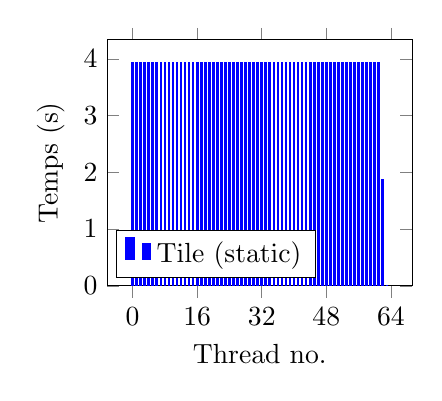
\begin{tikzpicture}
\begin{axis}[
  ybar,
  bar width=0.02cm,
  xlabel={Thread no.},
  ylabel={Temps (s)},
  ymin=0,
  legend pos=south west,
  width=0.45\textwidth,
  xtick distance=16
]

% Données pour le premier graphique (à gauche)
\addplot[color=blue, fill=blue] coordinates {
  (0,3.931419) (1,3.931297) (2,3.931273) (3,3.931255) (4,3.931230) (5,3.931260) (6,3.931294) (7,3.931271) (8,3.935328) (9,3.935309) (10,3.935331) (11,3.935283) (12,3.935421) (13,3.935430) (14,3.935398) (15,3.935381) (16,3.935664) (17,3.936624) (18,3.935655) (19,3.935715) (20,3.935612) (21,3.935455) (22,3.935500) (23,3.935588) (24,3.932591) (25,3.932589) (26,3.932618) (27,3.932659) (28,3.932749) (29,3.932762) (30,3.932788) (31,3.932710) (32,3.941319) (33,3.941172) (34,3.941358) (35,3.941352) (36,3.941333) (37,3.941382) (38,3.941428) (39,3.941422) (40,3.941497) (41,3.941570) (42,3.941579) (43,3.941611) (44,3.941558) (45,3.941591) (46,3.941622) (47,3.941593) (48,3.938724) (49,3.938698) (50,3.938737) (51,3.938801) (52,3.938822) (53,3.938817) (54,3.938870) (55,3.938896) (56,3.936364) (57,3.936303) (58,3.936332) (59,3.936368) (60,3.932841) (61,3.932937) (62,1.870698) (63,0.000073)
};
\addlegendentry{Tile (static)}

\end{axis}
\end{tikzpicture}
\hfill
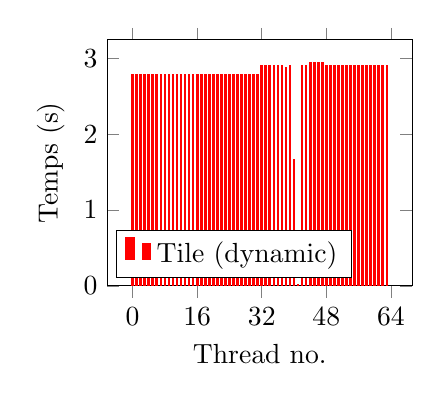
\begin{tikzpicture}
\begin{axis}[
  ybar,
  bar width=0.02cm,
  xlabel={Thread no.},
  ylabel={Temps (s)},
  ymin=0,
  legend pos=south west,
  width=0.45\textwidth,
  xtick distance=16
]

% Données pour le deuxième graphique (au milieu)
\addplot[color=red, fill=red] coordinates {
  (0,2.786878) (1,2.786835) (2,2.787426) (3,2.787119) (4,2.785719) (5,2.785795) (6,2.785832) (7,2.785830) (8,2.789159) (9,2.789159) (10,2.789170) (11,2.789145) (12,2.789059) (13,2.789098) (14,2.789086) (15,2.789092) (16,2.790921) (17,2.790885) (18,2.790961) (19,2.790942) (20,2.790962) (21,2.791071) (22,2.790907) (23,2.791267) (24,2.786639) (25,2.786603) (26,2.786613) (27,2.786660) (28,2.787449) (29,2.787451) (30,2.787404) (31,2.787471) (32,2.905044) (33,2.905006) (34,2.905050) (35,2.905045) (36,2.903501) (37,2.903458) (38,2.877404) (39,2.903528) (40,1.669344) (41,0.021980) (42,2.910888) (43,2.910928) (44,2.952890) (45,2.952885) (46,2.952917) (47,2.952927) (48,2.903597) (49,2.903365) (50,2.903602) (51,2.903604) (52,2.903366) (53,2.903408) (54,2.903615) (55,2.903608) (56,2.903459) (57,2.903520) (58,2.903551) (59,2.903577) (60,2.903372) (61,2.903430) (62,2.903587) (63,2.903606)
};
\addlegendentry{Tile (dynamic)}

\end{axis}
\end{tikzpicture}
\hfill
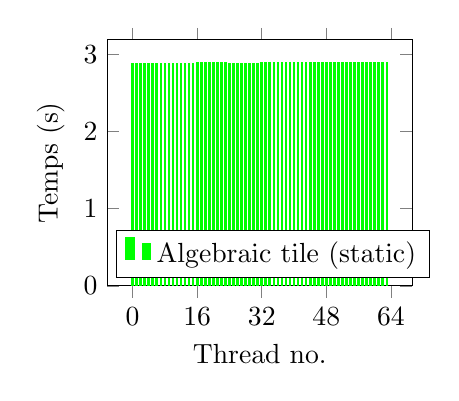
\begin{tikzpicture}
\begin{axis}[
  ybar,
  bar width=0.02cm,
  xlabel={Thread no.},
  ylabel={Temps (s)},
  ymin=0,
  legend pos=south west,
  width=0.45\textwidth,
  xtick distance=16
]

% Données pour le troisième graphique (à droite)
\addplot[color=green, fill=green] coordinates {
  (0,2.886257) (1,2.887295) (2,2.886337) (3,2.886364) (4,2.886047) (5,2.885984) (6,2.886054) (7,2.886058) (8,2.888761) (9,2.888753) (10,2.888798) (11,2.888749) (12,2.888732) (13,2.888679) (14,2.888750) (15,2.888670) (16,2.893684) (17,2.893731) (18,2.893705) (19,2.893698) (20,2.893431) (21,2.893345) (22,2.893463) (23,2.893429) (24,2.886786) (25,2.886845) (26,2.886826) (27,2.886765) (28,2.886933) (29,2.886918) (30,2.886933) (31,2.886921) (32,2.899985) (33,2.899835) (34,2.900135) (35,2.900222) (36,2.900165) (37,2.899802) (38,2.900132) (39,2.900180) (40,2.904274) (41,2.904105) (42,2.904282) (43,2.904270) (44,2.900208) (45,2.900265) (46,2.900518) (47,2.900535) (48,2.897410) (49,2.897588) (50,2.897889) (51,2.897727) (52,2.897652) (53,2.897614) (54,2.897672) (55,2.897870) (56,2.897749) (57,2.897853) (58,2.898017) (59,2.898038) (60,2.897574) (61,2.897514) (62,2.897899) (63,2.898002)
};
\addlegendentry{Algebraic tile (static)}

\end{axis}
\end{tikzpicture}

\caption{Temps d'exécution des threads pour le fichier gemm.c}
\label{fig:graphes}
\end{figure}

\begin{table}[htbp]
  \centering
  \caption{Statistiques pour le fichier gemm.c}
  \begin{tabular}{|c|c|c|c|}
    \hline
    Statistique & Algebraic Tile & Tile (static) & Tile (dynamic) \\ 
    \hline
    Skewness (g1)  & -0.0693501 & -6.11937 & -6.26377 \\ 
    Kurtosis (g2)  & -1.41896 & 37.4752 & 40.7194 \\ 
    Coefficient de variation $ \frac{\sigma}{\overline{x}} $ & 0.00202857 & 0.142539 & 0.137311\\ 
    Percent Imbalance metric en \% & 0.349392 & 2.57295 & 6.04302\\ 
    Coefficient de Gini  & 0.00114011 & 0.0242627 & 0.0327781\\ 
    Temps d'exécution (s) &  2.904415    &  3.946193   &  2.953131   \\ 

    \hline
  \end{tabular}
\end{table}
g1=$ \frac{\sum_{i=1}^{n} (x_i - \overline{x})^3}{n\sigma^3} $\
g2=$ \frac{\sum_{i=1}^{n} (x_i - \overline{x})^4}{n\sigma^4} $\
Coefficient de Gini = $ \frac{\sum_{i=1}^{n}\sum_{j=1}^{n} |x_i - x_j|}{2n^2\overline{x}} $\
\newpage

\begin{figure}
\centering

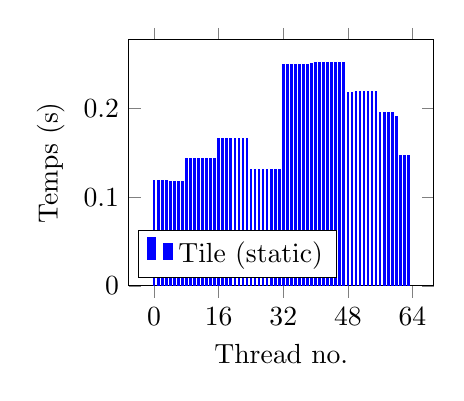
\begin{tikzpicture}
\begin{axis}[
  ybar,
  bar width=0.02cm,
  xlabel={Thread no.},
  ylabel={Temps (s)},
  ymin=0,
  legend pos=south west,
  width=0.45\textwidth,
  xtick distance=16
]

% Données pour le premier graphique (à gauche)
\addplot[color=blue, fill=blue] coordinates {
  (0,0.118435) (1,0.118190) (2,0.118178) (3,0.118185) (4,0.117794) (5,0.117792) (6,0.117777) (7,0.117782) (8,0.142958) (9,0.142964) (10,0.142999) (11,0.143099) (12,0.142996) (13,0.143115) (14,0.142987) (15,0.142988) (16,0.166043) (17,0.166045) (18,0.166040) (19,0.166043) (20,0.166169) (21,0.166169) (22,0.166171) (23,0.166168) (24,0.130962) (25,0.130960) (26,0.130960) (27,0.130969) (28,0.130995) (29,0.130986) (30,0.131000) (31,0.131002) (32,0.249643) (33,0.249942) (34,0.249859) (35,0.250019) (36,0.250087) (37,0.250062) (38,0.250081) (39,0.250124) (40,0.252209) (41,0.252207) (42,0.252266) (43,0.252264) (44,0.251963) (45,0.251858) (46,0.252163) (47,0.252176) (48,0.218470) (49,0.218497) (50,0.218661) (51,0.218620) (52,0.218789) (53,0.218801) (54,0.218817) (55,0.218799) (56,0.195143) (57,0.195122) (58,0.195297) (59,0.195293) (60,0.190445) (61,0.146926) (62,0.147149) (63,0.147141)
};
\addlegendentry{Tile (static)}

\end{axis}
\end{tikzpicture}
\hfill
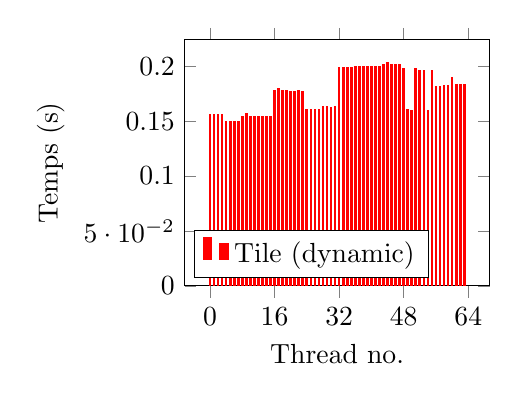
\begin{tikzpicture}
\begin{axis}[
  ybar,
  bar width=0.02cm,
  xlabel={Thread no.},
  ylabel={Temps (s)},
  ymin=0,
  legend pos=south west,
  width=0.45\textwidth,
  xtick distance=16
]

% Données pour le deuxième graphique (au milieu)
\addplot[color=red, fill=red] coordinates {
  (0,0.156023) (1,0.155932) (2,0.156033) (3,0.155987) (4,0.149356) (5,0.149346) (6,0.149702) (7,0.149346) (8,0.154098) (9,0.157216) (10,0.154108) (11,0.154091) (12,0.154350) (13,0.154368) (14,0.154335) (15,0.154346) (16,0.177518) (17,0.180152) (18,0.177518) (19,0.177542) (20,0.177221) (21,0.177221) (22,0.177582) (23,0.177227) (24,0.160192) (25,0.160188) (26,0.160190) (27,0.160243) (28,0.163148) (29,0.162921) (30,0.162700) (31,0.163031) (32,0.198766) (33,0.198918) (34,0.198895) (35,0.198795) (36,0.199327) (37,0.199338) (38,0.199327) (39,0.199357) (40,0.199669) (41,0.199579) (42,0.199698) (43,0.201860) (44,0.203783) (45,0.201673) (46,0.201611) (47,0.201601) (48,0.197842) (49,0.160967) (50,0.159581) (51,0.197849) (52,0.195857) (53,0.195763) (54,0.159562) (55,0.196015) (56,0.181901) (57,0.181898) (58,0.182095) (59,0.182128) (60,0.189400) (61,0.183469) (62,0.182954) (63,0.183075)
};
\addlegendentry{Tile (dynamic)}

\end{axis}
\end{tikzpicture}
\hfill
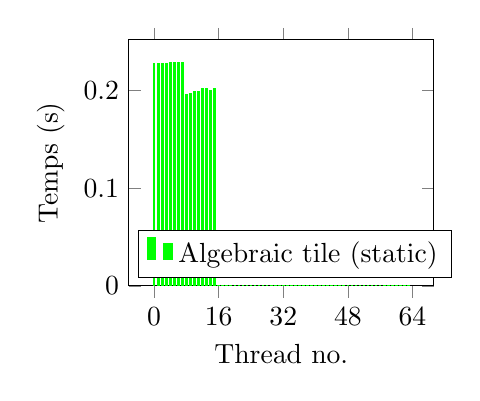
\begin{tikzpicture}
\begin{axis}[
  ybar,
  bar width=0.02cm,
  xlabel={Thread no.},
  ylabel={Temps (s)},
  ymin=0,
  legend pos=south west,
  width=0.45\textwidth,
  xtick distance=16
]

% Données pour le troisième graphique (à droite)
\addplot[color=green, fill=green] coordinates {
  (0,0.227389) (1,0.227546) (2,0.227750) (3,0.227805) (4,0.229047) (5,0.228328) (6,0.228199) (7,0.228193) (8,0.196283) (9,0.197363) (10,0.199119) (11,0.198866) (12,0.202058) (13,0.201972) (14,0.200115) (15,0.201853) (16,0.000238) (17,0.000237) (18,0.000237) (19,0.000237) (20,0.000238) (21,0.000238) (22,0.000238) (23,0.000238) (24,0.000242) (25,0.000242) (26,0.000242) (27,0.000242) (28,0.000235) (29,0.000236) (30,0.000235) (31,0.000235) (32,0.000228) (33,0.000227) (34,0.000228) (35,0.000227) (36,0.000232) (37,0.000233) (38,0.000233) (39,0.000233) (40,0.000233) (41,0.000233) (42,0.000233) (43,0.000233) (44,0.000238) (45,0.000238) (46,0.000238) (47,0.000238) (48,0.000233) (49,0.000234) (50,0.000233) (51,0.000233) (52,0.000233) (53,0.000233) (54,0.000233) (55,0.000233) (56,0.000236) (57,0.000236) (58,0.000236) (59,0.000236) (60,0.000235) (61,0.000235) (62,0.000235) (63,0.000235)
};
\addlegendentry{Algebraic tile (static)}

\end{axis}
\end{tikzpicture}

\caption{Temps d'exécution des threads pour le fichier gemver.c}
\label{fig:graphes}
\end{figure}

\begin{table}[htbp]
  \centering
  \caption{Statistiques pour le fichier gemver.c}
  \begin{tabular}{|c|c|c|c|}
    \hline
    Statistique & Algebraic Tile & Tile (static) & Tile (dynamic) \\ 
    \hline
    Skewness (g1)  & 1.17501 & 0.241278 & 0.0226222 \\ 
    Kurtosis (g2)  & -0.588698 & -1.50823 & -1.56962 \\ 
    Coefficient de variation $ \frac{\sigma}{\overline{x}} $ & 1.72956 & 0.274199 & 0.106169\\ 
    Percent Imbalance metric en \% & 326.982 & 38.6572 & 15.3578\\ 
    Coefficient de Gini  & 0.755397 & 0.154363 & 0.0600305\\ 
    Temps d'exécution (s) &  0.229499    &  0.252539   &  0.203949   \\ 

    \hline
  \end{tabular}
\end{table}
g1=$ \frac{\sum_{i=1}^{n} (x_i - \overline{x})^3}{n\sigma^3} $\
g2=$ \frac{\sum_{i=1}^{n} (x_i - \overline{x})^4}{n\sigma^4} $\
Coefficient de Gini = $ \frac{\sum_{i=1}^{n}\sum_{j=1}^{n} |x_i - x_j|}{2n^2\overline{x}} $\
\newpage

\begin{figure}
\centering

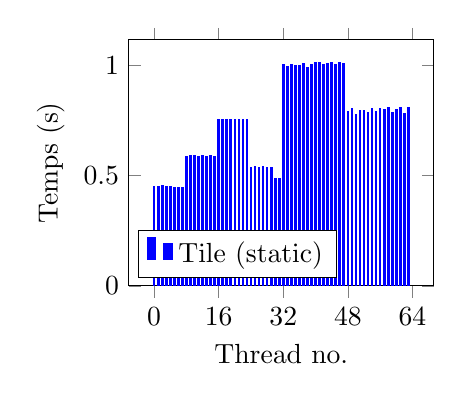
\begin{tikzpicture}
\begin{axis}[
  ybar,
  bar width=0.02cm,
  xlabel={Thread no.},
  ylabel={Temps (s)},
  ymin=0,
  legend pos=south west,
  width=0.45\textwidth,
  xtick distance=16
]

% Données pour le premier graphique (à gauche)
\addplot[color=blue, fill=blue] coordinates {
  (0,0.449522) (1,0.449111) (2,0.453943) (3,0.452758) (4,0.449924) (5,0.447436) (6,0.447436) (7,0.445827) (8,0.588493) (9,0.589550) (10,0.589523) (11,0.588041) (12,0.589626) (13,0.589196) (14,0.590067) (15,0.587910) (16,0.754248) (17,0.754087) (18,0.754542) (19,0.755002) (20,0.754592) (21,0.754853) (22,0.755153) (23,0.755309) (24,0.539395) (25,0.539579) (26,0.539421) (27,0.539599) (28,0.537076) (29,0.537324) (30,0.486059) (31,0.485794) (32,1.005131) (33,0.998360) (34,1.004541) (35,1.001432) (36,1.000725) (37,1.007600) (38,0.990436) (39,1.004852) (40,1.013829) (41,1.015942) (42,1.005839) (43,1.008721) (44,1.012378) (45,1.007069) (46,1.016316) (47,1.009020) (48,0.792577) (49,0.806661) (50,0.776287) (51,0.797014) (52,0.796154) (53,0.785140) (54,0.805677) (55,0.789780) (56,0.805166) (57,0.801075) (58,0.809772) (59,0.787072) (60,0.801019) (61,0.809716) (62,0.784240) (63,0.807770)
};
\addlegendentry{Tile (static)}

\end{axis}
\end{tikzpicture}
\hfill
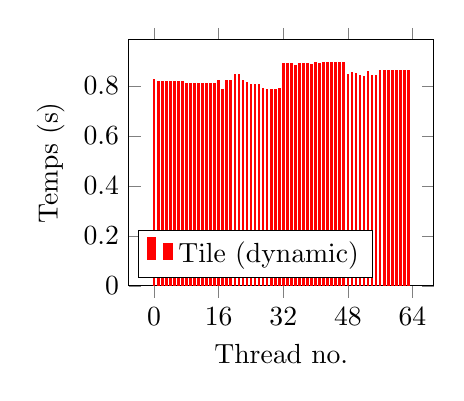
\begin{tikzpicture}
\begin{axis}[
  ybar,
  bar width=0.02cm,
  xlabel={Thread no.},
  ylabel={Temps (s)},
  ymin=0,
  legend pos=south west,
  width=0.45\textwidth,
  xtick distance=16
]

% Données pour le deuxième graphique (au milieu)
\addplot[color=red, fill=red] coordinates {
  (0,0.822947) (1,0.816356) (2,0.816115) (3,0.816211) (4,0.816719) (5,0.816809) (6,0.816380) (7,0.816803) (8,0.809173) (9,0.809530) (10,0.808531) (11,0.808840) (12,0.808206) (13,0.808638) (14,0.809612) (15,0.808659) (16,0.820295) (17,0.785747) (18,0.821172) (19,0.820175) (20,0.845993) (21,0.845813) (22,0.820473) (23,0.811587) (24,0.805670) (25,0.805691) (26,0.805697) (27,0.787905) (28,0.786827) (29,0.786625) (30,0.786512) (31,0.787684) (32,0.887567) (33,0.890011) (34,0.887397) (35,0.879475) (36,0.887831) (37,0.889629) (38,0.889408) (39,0.885831) (40,0.893041) (41,0.890537) (42,0.893273) (43,0.893914) (44,0.892744) (45,0.890943) (46,0.893689) (47,0.894654) (48,0.843716) (49,0.853985) (50,0.847942) (51,0.842917) (52,0.838535) (53,0.855233) (54,0.840254) (55,0.841517) (56,0.860642) (57,0.859520) (58,0.859698) (59,0.859822) (60,0.862100) (61,0.861941) (62,0.861871) (63,0.862617)
};
\addlegendentry{Tile (dynamic)}

\end{axis}
\end{tikzpicture}
\hfill
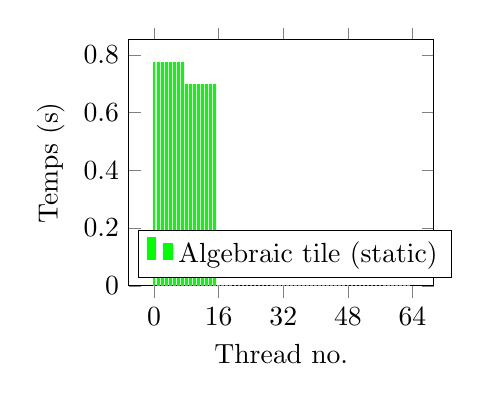
\begin{tikzpicture}
\begin{axis}[
  ybar,
  bar width=0.02cm,
  xlabel={Thread no.},
  ylabel={Temps (s)},
  ymin=0,
  legend pos=south west,
  width=0.45\textwidth,
  xtick distance=16
]

% Données pour le troisième graphique (à droite)
\addplot[color=green, fill=green] coordinates {
  (0,0.772530) (1,0.774675) (2,0.772135) (3,0.771869) (4,0.772255) (5,0.771984) (6,0.772348) (7,0.771869) (8,0.697644) (9,0.697737) (10,0.698230) (11,0.698414) (12,0.697111) (13,0.698032) (14,0.697841) (15,0.698406) (16,0.000259) (17,0.000259) (18,0.000259) (19,0.000259) (20,0.000257) (21,0.000257) (22,0.000257) (23,0.000257) (24,0.000254) (25,0.000254) (26,0.000254) (27,0.000255) (28,0.000257) (29,0.000257) (30,0.000257) (31,0.000257) (32,0.000245) (33,0.000245) (34,0.000245) (35,0.000245) (36,0.000245) (37,0.000245) (38,0.000245) (39,0.000245) (40,0.000249) (41,0.000248) (42,0.000248) (43,0.000248) (44,0.000249) (45,0.000249) (46,0.000249) (47,0.000249) (48,0.000247) (49,0.000247) (50,0.000247) (51,0.000248) (52,0.000245) (53,0.000245) (54,0.000245) (55,0.000245) (56,0.000249) (57,0.000249) (58,0.000249) (59,0.000249) (60,0.000255) (61,0.000256) (62,0.000256) (63,0.000256)
};
\addlegendentry{Algebraic tile (static)}

\end{axis}
\end{tikzpicture}

\caption{Temps d'exécution des threads pour le fichier gesummv.c}
\label{fig:graphes}
\end{figure}

\begin{table}[htbp]
  \centering
  \caption{Statistiques pour le fichier gesummv.c}
  \begin{tabular}{|c|c|c|c|}
    \hline
    Statistique & Algebraic Tile & Tile (static) & Tile (dynamic) \\ 
    \hline
    Skewness (g1)  & 1.16651 & -0.00967342 & 0.166289 \\ 
    Kurtosis (g2)  & -0.621235 & -1.24907 & -1.30299 \\ 
    Coefficient de variation $ \frac{\sigma}{\overline{x}} $ & 1.73265 & 0.262587 & 0.0417689\\ 
    Percent Imbalance metric en \% & 321.051 & 37.2019 & 6.3765\\ 
    Coefficient de Gini  & 0.755367 & 0.148051 & 0.0237404\\ 
    Temps d'exécution (s) &  0.774799    &  1.016626   &  0.895688   \\ 

    \hline
  \end{tabular}
\end{table}
g1=$ \frac{\sum_{i=1}^{n} (x_i - \overline{x})^3}{n\sigma^3} $\
g2=$ \frac{\sum_{i=1}^{n} (x_i - \overline{x})^4}{n\sigma^4} $\
Coefficient de Gini = $ \frac{\sum_{i=1}^{n}\sum_{j=1}^{n} |x_i - x_j|}{2n^2\overline{x}} $\
\newpage

\begin{figure}
\centering

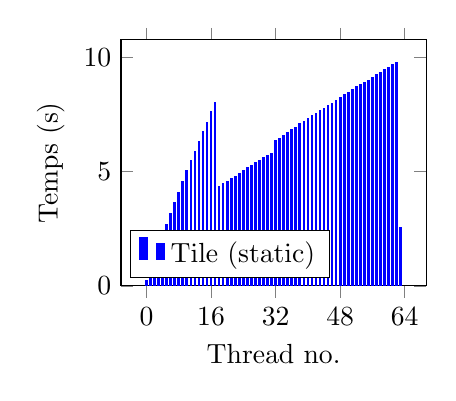
\begin{tikzpicture}
\begin{axis}[
  ybar,
  bar width=0.02cm,
  xlabel={Thread no.},
  ylabel={Temps (s)},
  ymin=0,
  legend pos=south west,
  width=0.45\textwidth,
  xtick distance=16
]

% Données pour le premier graphique (à gauche)
\addplot[color=blue, fill=blue] coordinates {
  (0,0.249792) (1,0.737683) (2,1.228964) (3,1.722346) (4,2.190033) (5,2.675652) (6,3.163810) (7,3.639137) (8,4.109263) (9,4.580493) (10,5.042366) (11,5.483083) (12,5.896786) (13,6.338358) (14,6.744623) (15,7.163123) (16,7.622295) (17,8.055822) (18,4.357130) (19,4.473799) (20,4.582098) (21,4.695567) (22,4.808147) (23,4.920272) (24,5.067578) (25,5.177024) (26,5.284652) (27,5.391529) (28,5.499925) (29,5.602643) (30,5.706941) (31,5.811233) (32,6.355842) (33,6.478099) (34,6.600131) (35,6.721882) (36,6.838607) (37,6.959340) (38,7.095764) (39,7.215695) (40,7.333637) (41,7.448552) (42,7.564458) (43,7.679152) (44,7.779033) (45,7.897523) (46,8.003735) (47,8.117985) (48,8.264515) (49,8.378524) (50,8.485324) (51,8.594488) (52,8.719268) (53,8.816418) (54,8.896140) (55,9.010028) (56,9.135638) (57,9.264172) (58,9.332440) (59,9.480808) (60,9.567903) (61,9.692360) (62,9.808387) (63,2.561010)
};
\addlegendentry{Tile (static)}

\end{axis}
\end{tikzpicture}
\hfill
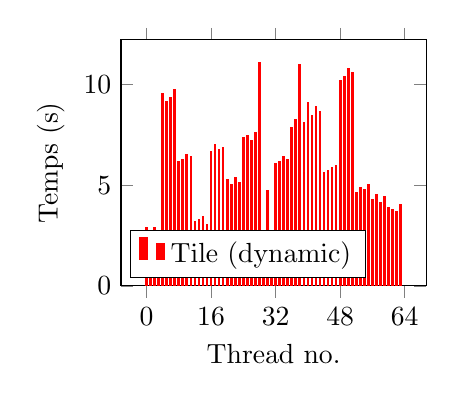
\begin{tikzpicture}
\begin{axis}[
  ybar,
  bar width=0.02cm,
  xlabel={Thread no.},
  ylabel={Temps (s)},
  ymin=0,
  legend pos=south west,
  width=0.45\textwidth,
  xtick distance=16
]

% Données pour le deuxième graphique (au milieu)
\addplot[color=red, fill=red] coordinates {
  (0,2.898047) (1,2.663326) (2,2.908379) (3,2.549531) (4,9.530993) (5,9.173432) (6,9.362927) (7,9.743440) (8,6.195327) (9,6.289294) (10,6.519768) (11,6.412425) (12,3.179943) (13,3.302526) (14,3.452123) (15,3.062029) (16,6.678013) (17,6.994352) (18,6.784163) (19,6.890723) (20,5.258770) (21,5.025034) (22,5.386515) (23,5.147462) (24,7.340166) (25,7.464776) (26,7.232905) (27,7.604010) (28,11.111226) (29,2.362692) (30,4.709254) (31,2.499426) (32,6.060866) (33,6.173595) (34,6.397749) (35,6.285711) (36,7.849001) (37,8.280152) (38,11.003249) (39,8.084953) (40,9.082024) (41,8.468489) (42,8.885846) (43,8.674190) (44,5.609371) (45,5.722628) (46,5.856189) (47,5.964541) (48,10.174617) (49,10.382695) (50,10.811176) (51,10.592093) (52,4.649760) (53,4.886480) (54,4.775323) (55,5.013758) (56,4.275981) (57,4.532800) (58,4.159864) (59,4.416783) (60,3.894404) (61,3.787776) (62,3.668539) (63,4.021416)
};
\addlegendentry{Tile (dynamic)}

\end{axis}
\end{tikzpicture}
\hfill
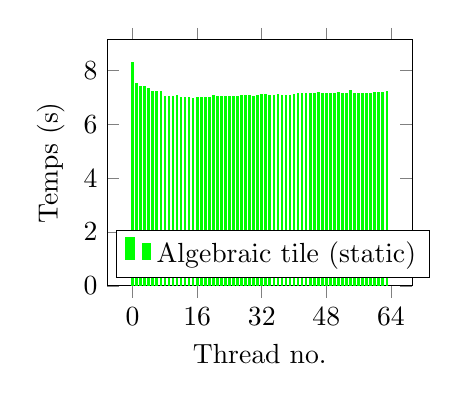
\begin{tikzpicture}
\begin{axis}[
  ybar,
  bar width=0.02cm,
  xlabel={Thread no.},
  ylabel={Temps (s)},
  ymin=0,
  legend pos=south west,
  width=0.45\textwidth,
  xtick distance=16
]

% Données pour le troisième graphique (à droite)
\addplot[color=green, fill=green] coordinates {
  (0,8.320749) (1,7.517609) (2,7.397176) (3,7.401786) (4,7.339777) (5,7.224490) (6,7.232399) (7,7.207992) (8,7.048620) (9,7.043628) (10,7.053196) (11,7.061834) (12,6.991090) (13,6.992928) (14,6.992854) (15,6.969320) (16,7.005304) (17,7.018513) (18,7.008527) (19,7.008528) (20,7.086193) (21,7.036582) (22,7.037336) (23,7.037347) (24,7.036302) (25,7.041230) (26,7.033682) (27,7.070685) (28,7.075770) (29,7.076018) (30,7.038173) (31,7.077417) (32,7.101319) (33,7.110222) (34,7.088559) (35,7.095215) (36,7.105388) (37,7.091961) (38,7.093342) (39,7.091977) (40,7.132817) (41,7.133115) (42,7.140962) (43,7.147212) (44,7.139539) (45,7.140043) (46,7.205651) (47,7.155642) (48,7.142691) (49,7.145450) (50,7.143464) (51,7.187317) (52,7.147742) (53,7.137221) (54,7.249866) (55,7.159651) (56,7.157921) (57,7.158866) (58,7.159257) (59,7.159948) (60,7.194752) (61,7.194017) (62,7.194474) (63,7.212525)
};
\addlegendentry{Algebraic tile (static)}

\end{axis}
\end{tikzpicture}

\caption{Temps d'exécution des threads pour le fichier syr2k.c}
\label{fig:graphes}
\end{figure}

\begin{table}[htbp]
  \centering
  \caption{Statistiques pour le fichier syr2k.c}
  \begin{tabular}{|c|c|c|c|}
    \hline
    Statistique & Algebraic Tile & Tile (static) & Tile (dynamic) \\ 
    \hline
    Skewness (g1)  & 4.54118 & -0.621619 & 0.325543 \\ 
    Kurtosis (g2)  & 26.2421 & -0.213442 & -0.833634 \\ 
    Coefficient de variation $ \frac{\sigma}{\overline{x}} $ & 0.0251626 & 0.37147 & 0.386638\\ 
    Percent Imbalance metric en \% & 16.4756 & 56.1072 & 78.5946\\ 
    Coefficient de Gini  & 0.00983766 & 0.208546 & 0.220977\\ 
    Temps d'exécution (s) &  8.329641    &  9.809628   &  11.115725   \\ 

    \hline
  \end{tabular}
\end{table}
g1=$ \frac{\sum_{i=1}^{n} (x_i - \overline{x})^3}{n\sigma^3} $\
g2=$ \frac{\sum_{i=1}^{n} (x_i - \overline{x})^4}{n\sigma^4} $\
Coefficient de Gini = $ \frac{\sum_{i=1}^{n}\sum_{j=1}^{n} |x_i - x_j|}{2n^2\overline{x}} $\
\newpage

\begin{figure}
\centering

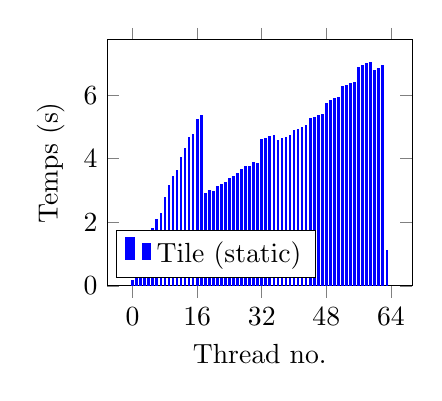
\begin{tikzpicture}
\begin{axis}[
  ybar,
  bar width=0.02cm,
  xlabel={Thread no.},
  ylabel={Temps (s)},
  ymin=0,
  legend pos=south west,
  width=0.45\textwidth,
  xtick distance=16
]

% Données pour le premier graphique (à gauche)
\addplot[color=blue, fill=blue] coordinates {
  (0,0.172136) (1,0.506631) (2,0.812637) (3,1.006176) (4,1.491156) (5,1.797595) (6,2.089946) (7,2.286161) (8,2.785890) (9,3.142867) (10,3.424371) (11,3.610896) (12,4.042126) (13,4.315958) (14,4.655013) (15,4.764831) (16,5.217064) (17,5.356469) (18,2.913468) (19,2.988568) (20,2.967436) (21,3.126542) (22,3.179758) (23,3.246000) (24,3.384688) (25,3.441820) (26,3.517130) (27,3.645258) (28,3.743446) (29,3.759624) (30,3.877890) (31,3.859247) (32,4.585767) (33,4.637882) (34,4.687982) (35,4.736662) (36,4.572971) (37,4.626223) (38,4.677160) (39,4.723518) (40,4.879089) (41,4.929896) (42,4.979447) (43,5.034992) (44,5.255405) (45,5.303143) (46,5.349146) (47,5.392752) (48,5.728103) (49,5.836546) (50,5.889673) (51,5.933363) (52,6.261224) (53,6.311111) (54,6.356038) (55,6.401298) (56,6.866694) (57,6.928865) (58,6.986426) (59,7.036918) (60,6.784840) (61,6.836790) (62,6.931142) (63,1.115055)
};
\addlegendentry{Tile (static)}

\end{axis}
\end{tikzpicture}
\hfill
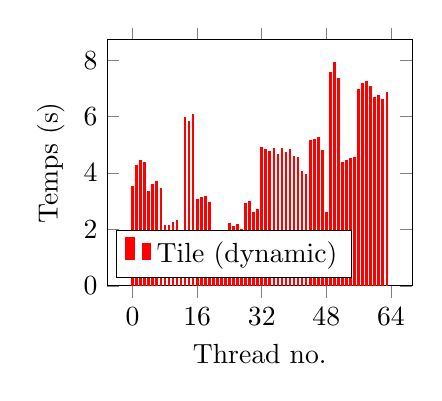
\begin{tikzpicture}
\begin{axis}[
  ybar,
  bar width=0.02cm,
  xlabel={Thread no.},
  ylabel={Temps (s)},
  ymin=0,
  legend pos=south west,
  width=0.45\textwidth,
  xtick distance=16
]

% Données pour le deuxième graphique (au milieu)
\addplot[color=red, fill=red] coordinates {
  (0,3.500087) (1,4.247181) (2,4.427680) (3,4.351059) (4,3.326934) (5,3.597209) (6,3.699414) (7,3.449865) (8,2.142719) (9,2.120395) (10,2.242895) (11,2.299986) (12,1.549301) (13,5.951428) (14,5.817951) (15,6.085847) (16,3.039828) (17,3.116341) (18,3.163047) (19,2.963627) (20,1.896044) (21,1.784461) (22,1.884589) (23,1.824251) (24,2.208751) (25,2.090121) (26,2.155030) (27,2.010018) (28,2.930742) (29,2.993736) (30,2.609302) (31,2.686724) (32,4.900915) (33,4.822331) (34,4.758904) (35,4.858442) (36,4.666238) (37,4.862793) (38,4.713778) (39,4.829893) (40,4.588926) (41,4.541590) (42,4.041582) (43,3.932913) (44,5.130826) (45,5.194327) (46,5.237887) (47,4.779381) (48,2.605643) (49,7.561881) (50,7.928109) (51,7.358570) (52,4.367568) (53,4.446672) (54,4.520643) (55,4.558071) (56,6.966263) (57,7.152907) (58,7.245006) (59,7.059032) (60,6.660339) (61,6.751136) (62,6.593118) (63,6.841006)
};
\addlegendentry{Tile (dynamic)}

\end{axis}
\end{tikzpicture}
\hfill
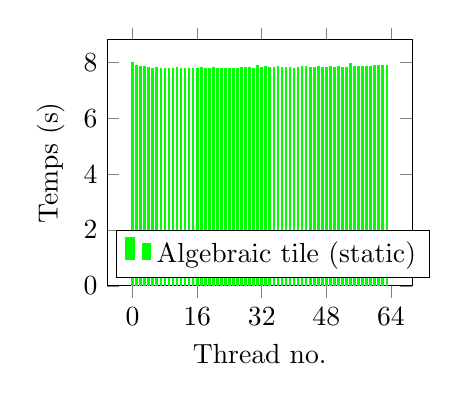
\begin{tikzpicture}
\begin{axis}[
  ybar,
  bar width=0.02cm,
  xlabel={Thread no.},
  ylabel={Temps (s)},
  ymin=0,
  legend pos=south west,
  width=0.45\textwidth,
  xtick distance=16
]

% Données pour le troisième graphique (à droite)
\addplot[color=green, fill=green] coordinates {
  (0,8.016737) (1,7.895718) (2,7.873692) (3,7.842596) (4,7.805464) (5,7.787593) (6,7.819023) (7,7.788769) (8,7.796106) (9,7.792995) (10,7.796290) (11,7.804888) (12,7.769842) (13,7.781970) (14,7.790877) (15,7.786586) (16,7.800420) (17,7.811785) (18,7.795293) (19,7.795251) (20,7.817547) (21,7.801435) (22,7.794873) (23,7.802567) (24,7.793647) (25,7.794701) (26,7.802040) (27,7.819957) (28,7.819534) (29,7.819569) (30,7.794848) (31,7.876728) (32,7.828467) (33,7.852814) (34,7.807952) (35,7.806311) (36,7.854972) (37,7.834481) (38,7.811222) (39,7.806154) (40,7.802957) (41,7.821804) (42,7.859413) (43,7.841507) (44,7.828638) (45,7.811029) (46,7.840317) (47,7.811244) (48,7.832710) (49,7.850585) (50,7.833213) (51,7.848954) (52,7.825798) (53,7.806963) (54,7.950418) (55,7.846038) (56,7.847387) (57,7.856505) (58,7.844605) (59,7.867483) (60,7.894286) (61,7.906557) (62,7.906612) (63,7.906744)
};
\addlegendentry{Algebraic tile (static)}

\end{axis}
\end{tikzpicture}

\caption{Temps d'exécution des threads pour le fichier syrk.c}
\label{fig:graphes}
\end{figure}

\begin{table}[htbp]
  \centering
  \caption{Statistiques pour le fichier syrk.c}
  \begin{tabular}{|c|c|c|c|}
    \hline
    Statistique & Algebraic Tile & Tile (static) & Tile (dynamic) \\ 
    \hline
    Skewness (g1)  & 1.79149 & -0.418508 & 0.329025 \\ 
    Kurtosis (g2)  & 4.32312 & -0.366596 & -0.86444 \\ 
    Coefficient de variation $ \frac{\sigma}{\overline{x}} $ & 0.00550691 & 0.398402 & 0.405296\\ 
    Percent Imbalance metric en \% & 2.38215 & 63.3495 & 86.1037\\ 
    Coefficient de Gini  & 0.00279572 & 0.224678 & 0.230479\\ 
    Temps d'exécution (s) &  8.025838    &  7.037140   &  7.930601   \\ 

    \hline
  \end{tabular}
\end{table}
g1=$ \frac{\sum_{i=1}^{n} (x_i - \overline{x})^3}{n\sigma^3} $\
g2=$ \frac{\sum_{i=1}^{n} (x_i - \overline{x})^4}{n\sigma^4} $\
Coefficient de Gini = $ \frac{\sum_{i=1}^{n}\sum_{j=1}^{n} |x_i - x_j|}{2n^2\overline{x}} $\
\newpage

\begin{figure}
\centering

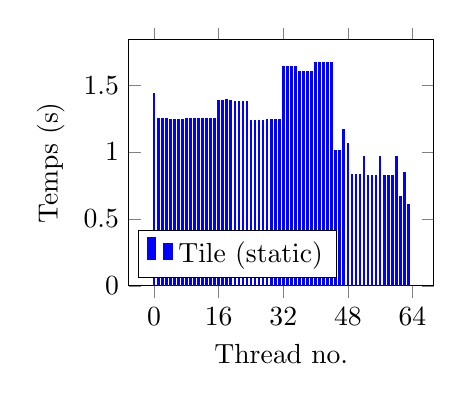
\begin{tikzpicture}
\begin{axis}[
  ybar,
  bar width=0.02cm,
  xlabel={Thread no.},
  ylabel={Temps (s)},
  ymin=0,
  legend pos=south west,
  width=0.45\textwidth,
  xtick distance=16
]

% Données pour le premier graphique (à gauche)
\addplot[color=blue, fill=blue] coordinates {
  (0,1.437462) (1,1.247034) (2,1.246998) (3,1.247069) (4,1.245447) (5,1.245510) (6,1.245572) (7,1.245489) (8,1.252800) (9,1.252921) (10,1.252911) (11,1.252939) (12,1.253111) (13,1.252838) (14,1.252894) (15,1.252905) (16,1.386511) (17,1.386508) (18,1.388873) (19,1.386544) (20,1.376627) (21,1.376486) (22,1.376686) (23,1.376568) (24,1.236957) (25,1.237042) (26,1.236964) (27,1.236937) (28,1.239732) (29,1.239856) (30,1.239836) (31,1.239817) (32,1.640780) (33,1.638696) (34,1.638638) (35,1.638703) (36,1.604020) (37,1.603962) (38,1.603974) (39,1.603985) (40,1.672212) (41,1.672026) (42,1.672050) (43,1.672338) (44,1.666531) (45,1.008751) (46,1.008645) (47,1.171414) (48,1.062987) (49,0.834062) (50,0.834751) (51,0.834094) (52,0.967204) (53,0.821107) (54,0.821348) (55,0.821341) (56,0.966777) (57,0.823804) (58,0.823050) (59,0.823027) (60,0.964038) (61,0.668034) (62,0.849849) (63,0.608380)
};
\addlegendentry{Tile (static)}

\end{axis}
\end{tikzpicture}
\hfill
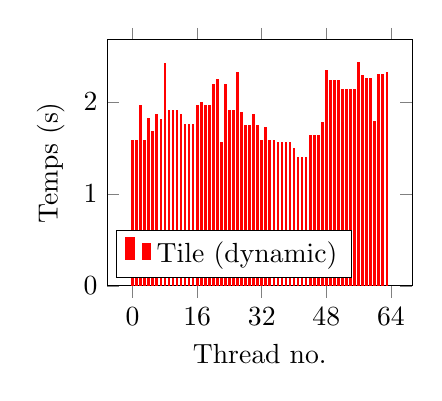
\begin{tikzpicture}
\begin{axis}[
  ybar,
  bar width=0.02cm,
  xlabel={Thread no.},
  ylabel={Temps (s)},
  ymin=0,
  legend pos=south west,
  width=0.45\textwidth,
  xtick distance=16
]

% Données pour le deuxième graphique (au milieu)
\addplot[color=red, fill=red] coordinates {
  (0,1.578140) (1,1.576525) (2,1.966535) (3,1.576577) (4,1.815158) (5,1.679973) (6,1.867215) (7,1.814959) (8,2.418469) (9,1.912447) (10,1.902708) (11,1.912430) (12,1.868195) (13,1.758987) (14,1.754736) (15,1.754687) (16,1.958965) (17,1.990346) (18,1.959110) (19,1.959072) (20,2.195674) (21,2.247181) (22,1.557869) (23,2.195681) (24,1.912022) (25,1.912058) (26,2.318416) (27,1.886557) (28,1.742523) (29,1.742686) (30,1.868147) (31,1.742539) (32,1.584215) (33,1.719068) (34,1.584167) (35,1.584151) (36,1.562631) (37,1.562513) (38,1.562577) (39,1.562654) (40,1.492701) (41,1.398256) (42,1.398327) (43,1.398300) (44,1.636401) (45,1.636346) (46,1.636421) (47,1.777028) (48,2.344120) (49,2.237366) (50,2.237347) (51,2.237284) (52,2.138204) (53,2.138120) (54,2.138256) (55,2.138202) (56,2.434633) (57,2.292608) (58,2.260051) (59,2.260045) (60,1.784049) (61,2.299939) (62,2.300227) (63,2.319185)
};
\addlegendentry{Tile (dynamic)}

\end{axis}
\end{tikzpicture}
\hfill
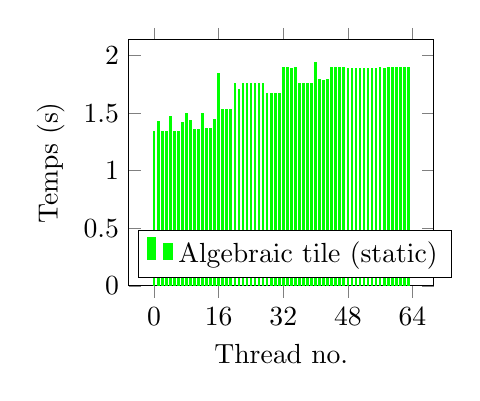
\begin{tikzpicture}
\begin{axis}[
  ybar,
  bar width=0.02cm,
  xlabel={Thread no.},
  ylabel={Temps (s)},
  ymin=0,
  legend pos=south west,
  width=0.45\textwidth,
  xtick distance=16
]

% Données pour le troisième graphique (à droite)
\addplot[color=green, fill=green] coordinates {
  (0,1.341574) (1,1.431036) (2,1.342621) (3,1.341688) (4,1.468680) (5,1.341886) (6,1.341892) (7,1.417855) (8,1.494332) (9,1.435832) (10,1.355196) (11,1.361421) (12,1.492883) (13,1.362431) (14,1.362332) (15,1.441326) (16,1.842877) (17,1.531429) (18,1.531408) (19,1.531335) (20,1.759480) (21,1.706990) (22,1.759562) (23,1.759603) (24,1.760550) (25,1.754896) (26,1.754996) (27,1.755096) (28,1.666360) (29,1.666400) (30,1.666385) (31,1.666236) (32,1.891876) (33,1.891880) (34,1.891797) (35,1.891879) (36,1.754903) (37,1.754953) (38,1.754896) (39,1.754952) (40,1.943378) (41,1.790485) (42,1.779519) (43,1.790688) (44,1.899242) (45,1.899234) (46,1.899247) (47,1.899253) (48,1.888155) (49,1.888126) (50,1.888244) (51,1.888305) (52,1.888604) (53,1.888637) (54,1.888771) (55,1.888763) (56,1.891945) (57,1.891859) (58,1.891987) (59,1.892003) (60,1.892709) (61,1.892617) (62,1.892862) (63,1.892910)
};
\addlegendentry{Algebraic tile (static)}

\end{axis}
\end{tikzpicture}

\caption{Temps d'exécution des threads pour le fichier trmm.c}
\label{fig:graphes}
\end{figure}

\begin{table}[htbp]
  \centering
  \caption{Statistiques pour le fichier trmm.c}
  \begin{tabular}{|c|c|c|c|}
    \hline
    Statistique & Algebraic Tile & Tile (static) & Tile (dynamic) \\ 
    \hline
    Skewness (g1)  & -0.678262 & -0.215335 & 0.189717 \\ 
    Kurtosis (g2)  & -1.07026 & -0.716517 & -1.12915 \\ 
    Coefficient de variation $ \frac{\sigma}{\overline{x}} $ & 0.119088 & 0.227816 & 0.152147\\ 
    Percent Imbalance metric en \% & 13.917 & 35.1614 & 28.7716\\ 
    Coefficient de Gini  & 0.0646509 & 0.126651 & 0.0869639\\ 
    Temps d'exécution (s) &  1.943920    &  1.673713   &  2.436635   \\ 

    \hline
  \end{tabular}
\end{table}
g1=$ \frac{\sum_{i=1}^{n} (x_i - \overline{x})^3}{n\sigma^3} $\
g2=$ \frac{\sum_{i=1}^{n} (x_i - \overline{x})^4}{n\sigma^4} $\
Coefficient de Gini = $ \frac{\sum_{i=1}^{n}\sum_{j=1}^{n} |x_i - x_j|}{2n^2\overline{x}} $\
\newpage

\begin{figure}
\centering

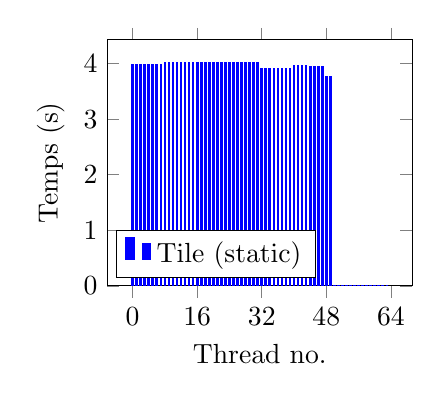
\begin{tikzpicture}
\begin{axis}[
  ybar,
  bar width=0.02cm,
  xlabel={Thread no.},
  ylabel={Temps (s)},
  ymin=0,
  legend pos=south west,
  width=0.45\textwidth,
  xtick distance=16
]

% Données pour le premier graphique (à gauche)
\addplot[color=blue, fill=blue] coordinates {
  (0,3.981750) (1,3.981465) (2,3.981582) (3,3.981602) (4,3.980855) (5,3.981014) (6,3.981078) (7,3.981016) (8,4.015645) (9,4.015692) (10,4.015664) (11,4.015695) (12,4.015621) (13,4.015620) (14,4.015659) (15,4.015642) (16,4.021712) (17,4.021720) (18,4.022021) (19,4.021657) (20,4.025058) (21,4.022397) (22,4.022375) (23,4.022417) (24,4.021109) (25,4.021248) (26,4.021219) (27,4.021001) (28,4.018224) (29,4.018668) (30,4.018669) (31,4.018915) (32,3.907245) (33,3.907390) (34,3.907451) (35,3.907442) (36,3.911441) (37,3.911376) (38,3.911527) (39,3.911388) (40,3.961095) (41,3.961093) (42,3.961216) (43,3.961175) (44,3.954210) (45,3.954173) (46,3.954282) (47,3.954312) (48,3.759748) (49,3.759714) (50,0.000063) (51,0.000062) (52,0.000063) (53,0.000061) (54,0.000062) (55,0.000061) (56,0.000064) (57,0.000063) (58,0.000063) (59,0.000064) (60,0.000064) (61,0.000064) (62,0.000064) (63,0.000064)
};
\addlegendentry{Tile (static)}

\end{axis}
\end{tikzpicture}
\hfill
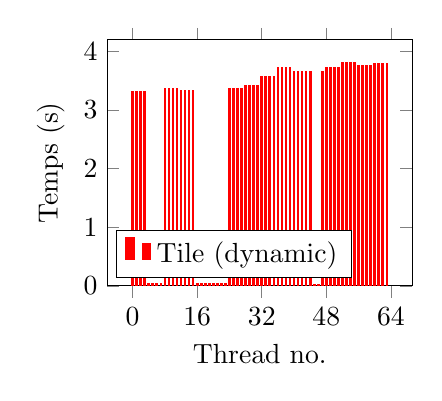
\begin{tikzpicture}
\begin{axis}[
  ybar,
  bar width=0.02cm,
  xlabel={Thread no.},
  ylabel={Temps (s)},
  ymin=0,
  legend pos=south west,
  width=0.45\textwidth,
  xtick distance=16
]

% Données pour le deuxième graphique (au milieu)
\addplot[color=red, fill=red] coordinates {
  (0,3.321219) (1,3.321196) (2,3.321241) (3,3.321193) (4,0.030225) (5,0.030130) (6,0.030282) (7,0.030073) (8,3.368772) (9,3.368689) (10,3.368693) (11,3.369300) (12,3.327235) (13,3.327207) (14,3.327212) (15,3.327230) (16,0.037213) (17,0.036889) (18,0.036909) (19,0.036911) (20,0.036856) (21,0.036841) (22,0.036860) (23,0.036845) (24,3.369057) (25,3.369011) (26,3.369002) (27,3.368972) (28,3.411226) (29,3.410718) (30,3.410688) (31,3.411448) (32,3.567734) (33,3.576613) (34,3.568469) (35,3.577106) (36,3.729072) (37,3.729072) (38,3.729088) (39,3.729088) (40,3.662676) (41,3.662676) (42,3.662676) (43,3.663350) (44,3.656147) (45,0.022354) (46,0.022463) (47,3.656147) (48,3.722380) (49,3.722339) (50,3.722331) (51,3.722330) (52,3.817806) (53,3.817827) (54,3.817834) (55,3.817868) (56,3.753724) (57,3.753201) (58,3.753236) (59,3.753304) (60,3.791829) (61,3.792043) (62,3.791806) (63,3.792400)
};
\addlegendentry{Tile (dynamic)}

\end{axis}
\end{tikzpicture}
\hfill
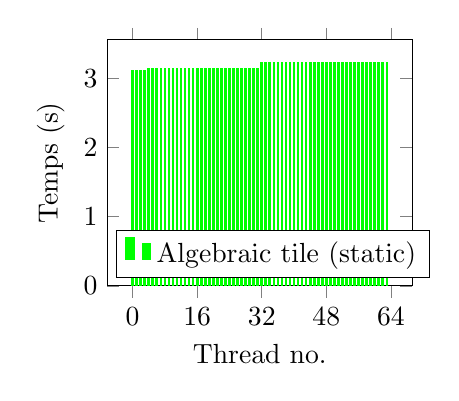
\begin{tikzpicture}
\begin{axis}[
  ybar,
  bar width=0.02cm,
  xlabel={Thread no.},
  ylabel={Temps (s)},
  ymin=0,
  legend pos=south west,
  width=0.45\textwidth,
  xtick distance=16
]

% Données pour le troisième graphique (à droite)
\addplot[color=green, fill=green] coordinates {
  (0,3.119540) (1,3.120095) (2,3.120111) (3,3.119981) (4,3.138139) (5,3.138177) (6,3.138103) (7,3.137933) (8,3.144882) (9,3.144693) (10,3.145011) (11,3.144867) (12,3.142057) (13,3.142025) (14,3.142043) (15,3.142066) (16,3.149488) (17,3.149535) (18,3.149506) (19,3.149500) (20,3.149733) (21,3.149698) (22,3.149717) (23,3.149732) (24,3.143806) (25,3.143932) (26,3.143904) (27,3.144012) (28,3.146564) (29,3.146546) (30,3.146563) (31,3.146605) (32,3.235856) (33,3.235815) (34,3.235731) (35,3.235806) (36,3.235867) (37,3.235879) (38,3.235853) (39,3.235872) (40,3.238037) (41,3.237921) (42,3.238071) (43,3.238088) (44,3.237448) (45,3.237423) (46,3.237470) (47,3.237465) (48,3.232141) (49,3.232129) (50,3.232009) (51,3.232062) (52,3.231726) (53,3.231865) (54,3.231682) (55,3.231769) (56,3.232095) (57,3.232039) (58,3.232127) (59,3.231994) (60,3.229329) (61,3.229782) (62,3.229841) (63,3.229774)
};
\addlegendentry{Algebraic tile (static)}

\end{axis}
\end{tikzpicture}

\caption{Temps d'exécution des threads pour le fichier 2mm.c}
\label{fig:graphes}
\end{figure}

\begin{table}[htbp]
  \centering
  \caption{Statistiques pour le fichier 2mm.c}
  \begin{tabular}{|c|c|c|c|}
    \hline
    Statistique & Algebraic Tile & Tile (static) & Tile (dynamic) \\ 
    \hline
    Skewness (g1)  & -0.0557961 & -1.35703 & -1.31602 \\ 
    Kurtosis (g2)  & -1.89337 & -0.152834 & -0.198717 \\ 
    Coefficient de variation $ \frac{\sigma}{\overline{x}} $ & 0.014622 & 0.529409 & 0.526214\\ 
    Percent Imbalance metric en \% & 1.57242 & 29.5981 & 36.3812\\ 
    Coefficient de Gini  & 0.00770422 & 0.224416 & 0.238855\\ 
    Temps d'exécution (s) &  3.238915    &  4.028952   &  3.818190   \\ 

    \hline
  \end{tabular}
\end{table}
g1=$ \frac{\sum_{i=1}^{n} (x_i - \overline{x})^3}{n\sigma^3} $\
g2=$ \frac{\sum_{i=1}^{n} (x_i - \overline{x})^4}{n\sigma^4} $\
Coefficient de Gini = $ \frac{\sum_{i=1}^{n}\sum_{j=1}^{n} |x_i - x_j|}{2n^2\overline{x}} $\
\newpage

\begin{figure}
\centering

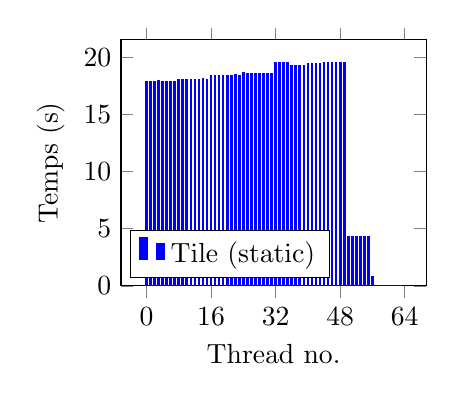
\begin{tikzpicture}
\begin{axis}[
  ybar,
  bar width=0.02cm,
  xlabel={Thread no.},
  ylabel={Temps (s)},
  ymin=0,
  legend pos=south west,
  width=0.45\textwidth,
  xtick distance=16
]

% Données pour le premier graphique (à gauche)
\addplot[color=blue, fill=blue] coordinates {
  (0,17.911004) (1,17.910610) (2,17.910704) (3,17.946427) (4,17.911218) (5,17.911224) (6,17.911271) (7,17.911169) (8,18.088303) (9,18.088298) (10,18.088257) (11,18.088324) (12,18.088518) (13,18.088532) (14,18.118195) (15,18.088479) (16,18.405956) (17,18.405980) (18,18.405999) (19,18.405846) (20,18.406239) (21,18.406007) (22,18.490638) (23,18.405798) (24,18.660819) (25,18.636824) (26,18.637008) (27,18.636914) (28,18.612779) (29,18.609005) (30,18.609135) (31,18.609110) (32,19.539474) (33,19.539542) (34,19.539563) (35,19.539446) (36,19.289003) (37,19.288983) (38,19.288995) (39,19.288932) (40,19.431544) (41,19.431562) (42,19.431555) (43,19.431626) (44,19.577796) (45,19.578105) (46,19.578072) (47,19.578073) (48,19.595582) (49,19.595693) (50,4.354156) (51,4.354156) (52,4.324260) (53,4.324260) (54,4.324261) (55,4.324260) (56,0.800156) (57,0.000204) (58,0.000204) (59,0.000205) (60,0.000203) (61,0.000204) (62,0.000203) (63,0.000204)
};
\addlegendentry{Tile (static)}

\end{axis}
\end{tikzpicture}
\hfill
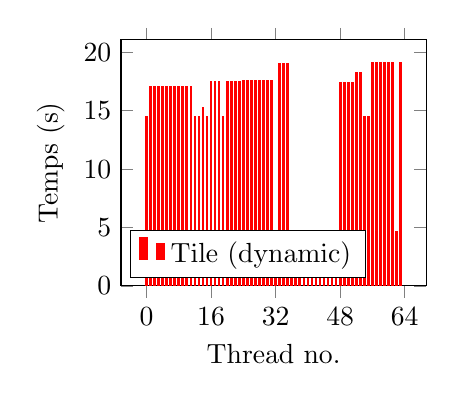
\begin{tikzpicture}
\begin{axis}[
  ybar,
  bar width=0.02cm,
  xlabel={Thread no.},
  ylabel={Temps (s)},
  ymin=0,
  legend pos=south west,
  width=0.45\textwidth,
  xtick distance=16
]

% Données pour le deuxième graphique (au milieu)
\addplot[color=red, fill=red] coordinates {
  (0,14.515018) (1,17.096789) (2,17.096698) (3,17.096822) (4,17.096496) (5,17.096360) (6,17.096566) (7,17.096161) (8,17.081689) (9,17.099148) (10,17.098927) (11,17.098838) (12,14.516597) (13,14.516763) (14,15.238131) (15,14.516662) (16,17.492281) (17,17.492313) (18,17.472884) (19,14.500445) (20,17.495122) (21,17.495346) (22,17.495411) (23,17.495433) (24,17.570802) (25,17.570525) (26,17.570638) (27,17.570655) (28,17.570904) (29,17.571349) (30,17.570414) (31,17.570678) (32,4.613657) (33,19.065643) (34,19.065001) (35,19.065070) (36,4.557300) (37,4.563636) (38,4.557300) (39,4.557300) (40,4.192104) (41,4.191984) (42,4.192122) (43,4.192083) (44,2.707641) (45,2.707653) (46,2.707387) (47,2.707466) (48,17.413370) (49,17.390534) (50,17.407473) (51,17.407856) (52,18.252079) (53,18.252265) (54,14.512585) (55,14.512817) (56,19.162966) (57,19.164071) (58,19.162919) (59,19.162993) (60,19.139818) (61,19.140401) (62,4.680947) (63,19.140611)
};
\addlegendentry{Tile (dynamic)}

\end{axis}
\end{tikzpicture}
\hfill
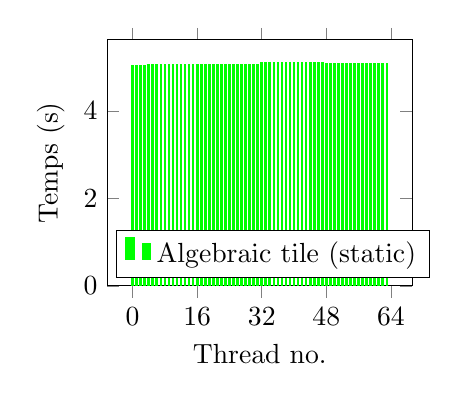
\begin{tikzpicture}
\begin{axis}[
  ybar,
  bar width=0.02cm,
  xlabel={Thread no.},
  ylabel={Temps (s)},
  ymin=0,
  legend pos=south west,
  width=0.45\textwidth,
  xtick distance=16
]

% Données pour le troisième graphique (à droite)
\addplot[color=green, fill=green] coordinates {
  (0,5.039535) (1,5.040649) (2,5.039838) (3,5.040023) (4,5.065473) (5,5.065309) (6,5.065419) (7,5.065324) (8,5.065576) (9,5.065719) (10,5.065702) (11,5.065719) (12,5.065862) (13,5.065830) (14,5.065908) (15,5.065808) (16,5.065273) (17,5.064874) (18,5.065283) (19,5.065051) (20,5.065231) (21,5.065116) (22,5.065382) (23,5.065291) (24,5.065487) (25,5.065476) (26,5.065449) (27,5.065593) (28,5.065761) (29,5.065552) (30,5.065770) (31,5.065521) (32,5.117938) (33,5.117807) (34,5.117779) (35,5.117586) (36,5.116925) (37,5.116687) (38,5.117019) (39,5.116806) (40,5.120827) (41,5.120783) (42,5.120655) (43,5.120607) (44,5.118809) (45,5.118727) (46,5.118680) (47,5.118715) (48,5.085587) (49,5.085830) (50,5.085745) (51,5.085725) (52,5.084329) (53,5.084668) (54,5.084434) (55,5.084527) (56,5.088299) (57,5.088459) (58,5.088545) (59,5.088097) (60,5.084549) (61,5.084666) (62,5.084438) (63,5.084743)
};
\addlegendentry{Algebraic tile (static)}

\end{axis}
\end{tikzpicture}

\caption{Temps d'exécution des threads pour le fichier 3mm.c}
\label{fig:graphes}
\end{figure}

\begin{table}[htbp]
  \centering
  \caption{Statistiques pour le fichier 3mm.c}
  \begin{tabular}{|c|c|c|c|}
    \hline
    Statistique & Algebraic Tile & Tile (static) & Tile (dynamic) \\ 
    \hline
    Skewness (g1)  & 0.38937 & -1.40666 & -1.22008 \\ 
    Kurtosis (g2)  & -0.917304 & 0.116383 & -0.273485 \\ 
    Coefficient de variation $ \frac{\sigma}{\overline{x}} $ & 0.00468773 & 0.467804 & 0.394359\\ 
    Percent Imbalance metric en \% & 0.75945 & 30.3998 & 33.2559\\ 
    Coefficient de Gini  & 0.00252531 & 0.208522 & 0.190572\\ 
    Temps d'exécution (s) &  5.129881    &  19.656638   &  19.173317   \\ 

    \hline
  \end{tabular}
\end{table}
g1=$ \frac{\sum_{i=1}^{n} (x_i - \overline{x})^3}{n\sigma^3} $\
g2=$ \frac{\sum_{i=1}^{n} (x_i - \overline{x})^4}{n\sigma^4} $\
Coefficient de Gini = $ \frac{\sum_{i=1}^{n}\sum_{j=1}^{n} |x_i - x_j|}{2n^2\overline{x}} $\
\newpage

\begin{figure}
\centering

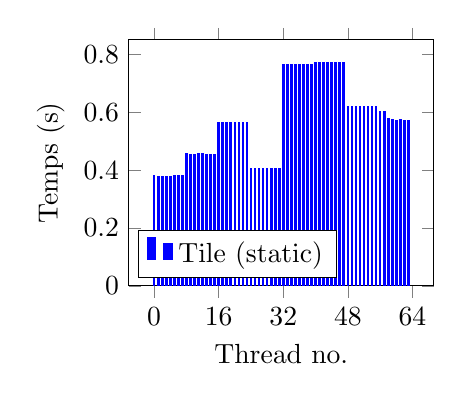
\begin{tikzpicture}
\begin{axis}[
  ybar,
  bar width=0.02cm,
  xlabel={Thread no.},
  ylabel={Temps (s)},
  ymin=0,
  legend pos=south west,
  width=0.45\textwidth,
  xtick distance=16
]

% Données pour le premier graphique (à gauche)
\addplot[color=blue, fill=blue] coordinates {
  (0,0.382966) (1,0.377669) (2,0.377929) (3,0.377646) (4,0.378892) (5,0.381777) (6,0.380803) (7,0.380602) (8,0.456487) (9,0.455953) (10,0.455480) (11,0.456433) (12,0.456135) (13,0.454812) (14,0.454993) (15,0.452768) (16,0.564749) (17,0.566751) (18,0.564768) (19,0.564852) (20,0.563996) (21,0.564033) (22,0.563925) (23,0.563972) (24,0.405623) (25,0.405566) (26,0.405473) (27,0.405593) (28,0.407048) (29,0.407156) (30,0.407098) (31,0.407288) (32,0.766276) (33,0.765827) (34,0.765805) (35,0.765800) (36,0.765865) (37,0.764692) (38,0.767113) (39,0.764570) (40,0.772663) (41,0.772561) (42,0.772797) (43,0.773153) (44,0.773296) (45,0.773196) (46,0.774250) (47,0.773309) (48,0.619225) (49,0.618963) (50,0.620277) (51,0.620942) (52,0.622168) (53,0.620888) (54,0.621572) (55,0.621345) (56,0.601568) (57,0.601653) (58,0.577255) (59,0.576538) (60,0.573381) (61,0.573917) (62,0.573574) (63,0.571601)
};
\addlegendentry{Tile (static)}

\end{axis}
\end{tikzpicture}
\hfill
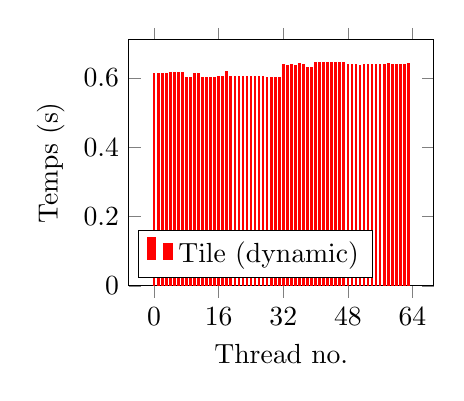
\begin{tikzpicture}
\begin{axis}[
  ybar,
  bar width=0.02cm,
  xlabel={Thread no.},
  ylabel={Temps (s)},
  ymin=0,
  legend pos=south west,
  width=0.45\textwidth,
  xtick distance=16
]

% Données pour le deuxième graphique (au milieu)
\addplot[color=red, fill=red] coordinates {
  (0,0.612181) (1,0.612461) (2,0.612059) (3,0.612314) (4,0.615651) (5,0.615377) (6,0.615421) (7,0.615179) (8,0.601486) (9,0.601876) (10,0.613353) (11,0.613200) (12,0.601130) (13,0.601054) (14,0.600157) (15,0.600347) (16,0.603803) (17,0.603566) (18,0.618571) (19,0.603897) (20,0.604808) (21,0.604851) (22,0.604854) (23,0.605074) (24,0.604508) (25,0.604551) (26,0.604513) (27,0.604613) (28,0.602569) (29,0.602663) (30,0.602695) (31,0.602567) (32,0.638576) (33,0.635319) (34,0.638959) (35,0.636025) (36,0.640554) (37,0.638886) (38,0.629187) (39,0.629326) (40,0.644613) (41,0.644756) (42,0.644964) (43,0.645526) (44,0.645352) (45,0.645185) (46,0.645840) (47,0.645345) (48,0.639211) (49,0.639524) (50,0.639419) (51,0.635597) (52,0.639512) (53,0.639183) (54,0.637600) (55,0.639048) (56,0.640097) (57,0.638968) (58,0.640397) (59,0.637964) (60,0.640044) (61,0.638100) (62,0.639810) (63,0.640622)
};
\addlegendentry{Tile (dynamic)}

\end{axis}
\end{tikzpicture}
\hfill
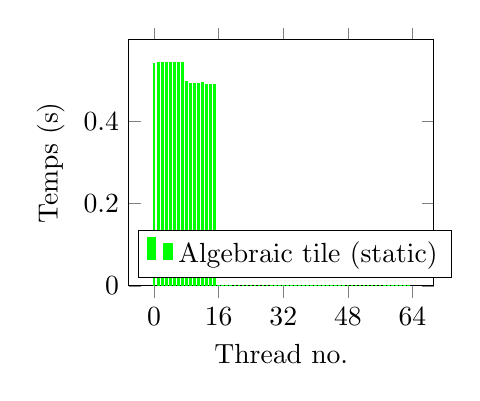
\begin{tikzpicture}
\begin{axis}[
  ybar,
  bar width=0.02cm,
  xlabel={Thread no.},
  ylabel={Temps (s)},
  ymin=0,
  legend pos=south west,
  width=0.45\textwidth,
  xtick distance=16
]

% Données pour le troisième graphique (à droite)
\addplot[color=green, fill=green] coordinates {
  (0,0.541885) (1,0.544362) (2,0.544740) (3,0.543809) (4,0.544823) (5,0.544586) (6,0.544237) (7,0.543871) (8,0.497758) (9,0.491582) (10,0.491912) (11,0.491714) (12,0.495571) (13,0.491056) (14,0.490976) (15,0.491267) (16,0.000168) (17,0.000166) (18,0.000166) (19,0.000165) (20,0.000172) (21,0.000171) (22,0.000172) (23,0.000172) (24,0.000168) (25,0.000166) (26,0.000166) (27,0.000167) (28,0.000169) (29,0.000168) (30,0.000168) (31,0.000168) (32,0.000155) (33,0.000160) (34,0.000158) (35,0.000160) (36,0.000156) (37,0.000154) (38,0.000154) (39,0.000154) (40,0.000163) (41,0.000164) (42,0.000162) (43,0.000163) (44,0.000162) (45,0.000157) (46,0.000162) (47,0.000162) (48,0.000158) (49,0.000158) (50,0.000157) (51,0.000157) (52,0.000158) (53,0.000160) (54,0.000158) (55,0.000158) (56,0.000161) (57,0.000162) (58,0.000160) (59,0.000159) (60,0.000163) (61,0.000160) (62,0.000160) (63,0.000163)
};
\addlegendentry{Algebraic tile (static)}

\end{axis}
\end{tikzpicture}

\caption{Temps d'exécution des threads pour le fichier atax.c}
\label{fig:graphes}
\end{figure}

\begin{table}[htbp]
  \centering
  \caption{Statistiques pour le fichier atax.c}
  \begin{tabular}{|c|c|c|c|}
    \hline
    Statistique & Algebraic Tile & Tile (static) & Tile (dynamic) \\ 
    \hline
    Skewness (g1)  & 1.16601 & 0.180492 & -0.0619433 \\ 
    Kurtosis (g2)  & -0.623182 & -1.28051 & -1.7525 \\ 
    Coefficient de variation $ \frac{\sigma}{\overline{x}} $ & 1.73272 & 0.247681 & 0.0274932\\ 
    Percent Imbalance metric en \% & 320.006 & 36.2243 & 3.60676\\ 
    Coefficient de Gini  & 0.755442 & 0.139446 & 0.0152477\\ 
    Temps d'exécution (s) &  0.545468    &  0.774464   &  0.652932   \\ 

    \hline
  \end{tabular}
\end{table}
g1=$ \frac{\sum_{i=1}^{n} (x_i - \overline{x})^3}{n\sigma^3} $\
g2=$ \frac{\sum_{i=1}^{n} (x_i - \overline{x})^4}{n\sigma^4} $\
Coefficient de Gini = $ \frac{\sum_{i=1}^{n}\sum_{j=1}^{n} |x_i - x_j|}{2n^2\overline{x}} $\
\newpage

\begin{figure}
\centering

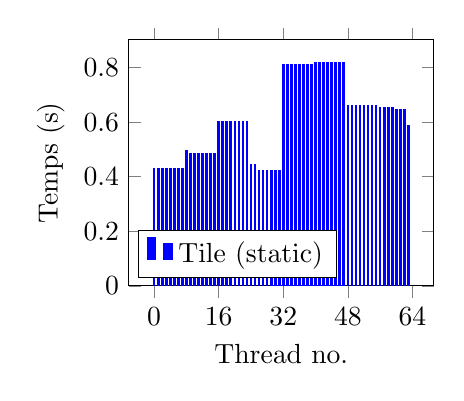
\begin{tikzpicture}
\begin{axis}[
  ybar,
  bar width=0.02cm,
  xlabel={Thread no.},
  ylabel={Temps (s)},
  ymin=0,
  legend pos=south west,
  width=0.45\textwidth,
  xtick distance=16
]

% Données pour le premier graphique (à gauche)
\addplot[color=blue, fill=blue] coordinates {
  (0,0.429726) (1,0.428661) (2,0.428666) (3,0.428660) (4,0.428073) (5,0.428141) (6,0.428104) (7,0.428144) (8,0.494589) (9,0.486140) (10,0.486184) (11,0.486401) (12,0.485917) (13,0.486216) (14,0.486081) (15,0.486267) (16,0.602319) (17,0.602411) (18,0.602424) (19,0.602361) (20,0.602334) (21,0.602316) (22,0.602271) (23,0.602344) (24,0.446028) (25,0.445978) (26,0.422862) (27,0.422906) (28,0.423836) (29,0.423865) (30,0.423958) (31,0.423975) (32,0.812632) (33,0.812630) (34,0.812562) (35,0.812645) (36,0.812191) (37,0.812354) (38,0.812484) (39,0.812873) (40,0.819763) (41,0.819806) (42,0.820003) (43,0.819611) (44,0.820021) (45,0.819801) (46,0.819587) (47,0.820071) (48,0.659687) (49,0.659243) (50,0.659453) (51,0.659216) (52,0.659359) (53,0.659380) (54,0.659458) (55,0.659753) (56,0.654363) (57,0.654611) (58,0.654739) (59,0.654703) (60,0.647012) (61,0.646978) (62,0.647107) (63,0.585982)
};
\addlegendentry{Tile (static)}

\end{axis}
\end{tikzpicture}
\hfill
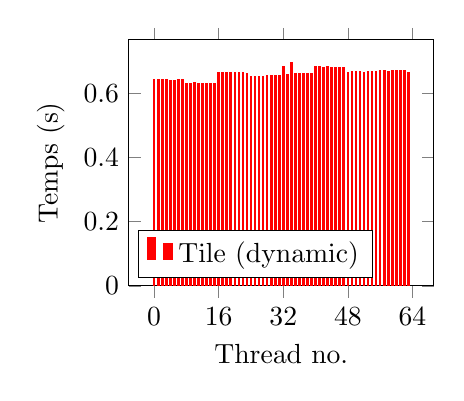
\begin{tikzpicture}
\begin{axis}[
  ybar,
  bar width=0.02cm,
  xlabel={Thread no.},
  ylabel={Temps (s)},
  ymin=0,
  legend pos=south west,
  width=0.45\textwidth,
  xtick distance=16
]

% Données pour le deuxième graphique (au milieu)
\addplot[color=red, fill=red] coordinates {
  (0,0.642026) (1,0.642031) (2,0.642520) (3,0.642506) (4,0.640749) (5,0.640712) (6,0.641064) (7,0.640819) (8,0.629486) (9,0.630273) (10,0.631538) (11,0.630679) (12,0.630359) (13,0.630316) (14,0.630348) (15,0.630580) (16,0.663653) (17,0.663075) (18,0.663643) (19,0.663074) (20,0.662734) (21,0.663231) (22,0.662688) (23,0.662583) (24,0.652584) (25,0.652556) (26,0.652586) (27,0.652732) (28,0.653645) (29,0.653781) (30,0.653646) (31,0.653819) (32,0.683573) (33,0.659243) (34,0.696645) (35,0.660123) (36,0.661552) (37,0.661709) (38,0.661667) (39,0.661943) (40,0.681398) (41,0.683669) (42,0.680952) (43,0.681761) (44,0.679797) (45,0.680254) (46,0.680455) (47,0.680158) (48,0.664934) (49,0.667043) (50,0.667440) (51,0.668259) (52,0.664037) (53,0.667273) (54,0.667883) (55,0.667815) (56,0.669362) (57,0.670108) (58,0.666920) (59,0.670119) (60,0.669179) (61,0.670398) (62,0.670311) (63,0.665294)
};
\addlegendentry{Tile (dynamic)}

\end{axis}
\end{tikzpicture}
\hfill
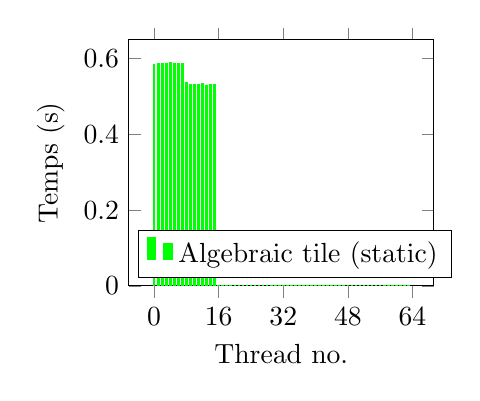
\begin{tikzpicture}
\begin{axis}[
  ybar,
  bar width=0.02cm,
  xlabel={Thread no.},
  ylabel={Temps (s)},
  ymin=0,
  legend pos=south west,
  width=0.45\textwidth,
  xtick distance=16
]

% Données pour le troisième graphique (à droite)
\addplot[color=green, fill=green] coordinates {
  (0,0.585059) (1,0.586421) (2,0.586692) (3,0.587123) (4,0.591079) (5,0.586811) (6,0.586999) (7,0.586823) (8,0.535823) (9,0.531346) (10,0.531410) (11,0.531497) (12,0.535091) (13,0.530009) (14,0.530589) (15,0.530761) (16,0.000163) (17,0.000162) (18,0.000162) (19,0.000162) (20,0.000165) (21,0.000165) (22,0.000165) (23,0.000165) (24,0.000162) (25,0.000164) (26,0.000162) (27,0.000163) (28,0.000163) (29,0.000162) (30,0.000162) (31,0.000163) (32,0.000160) (33,0.000159) (34,0.000160) (35,0.000160) (36,0.000158) (37,0.000158) (38,0.000159) (39,0.000159) (40,0.000164) (41,0.000162) (42,0.000164) (43,0.000163) (44,0.000164) (45,0.000163) (46,0.000164) (47,0.000164) (48,0.000159) (49,0.000159) (50,0.000159) (51,0.000159) (52,0.000158) (53,0.000157) (54,0.000158) (55,0.000157) (56,0.000162) (57,0.000161) (58,0.000162) (59,0.000161) (60,0.000160) (61,0.000159) (62,0.000160) (63,0.000159)
};
\addlegendentry{Algebraic tile (static)}

\end{axis}
\end{tikzpicture}

\caption{Temps d'exécution des threads pour le fichier bicg.c}
\label{fig:graphes}
\end{figure}

\begin{table}[htbp]
  \centering
  \caption{Statistiques pour le fichier bicg.c}
  \begin{tabular}{|c|c|c|c|}
    \hline
    Statistique & Algebraic Tile & Tile (static) & Tile (dynamic) \\ 
    \hline
    Skewness (g1)  & 1.16588 & 0.153091 & -0.265863 \\ 
    Kurtosis (g2)  & -0.623692 & -1.33098 & -0.561668 \\ 
    Coefficient de variation $ \frac{\sigma}{\overline{x}} $ & 1.73286 & 0.238824 & 0.0244696\\ 
    Percent Imbalance metric en \% & 322.139 & 34.3751 & 5.68406\\ 
    Coefficient de Gini  & 0.755481 & 0.134147 & 0.0136829\\ 
    Temps d'exécution (s) &  0.591976    &  0.820335   &  0.698561   \\ 

    \hline
  \end{tabular}
\end{table}
g1=$ \frac{\sum_{i=1}^{n} (x_i - \overline{x})^3}{n\sigma^3} $\
g2=$ \frac{\sum_{i=1}^{n} (x_i - \overline{x})^4}{n\sigma^4} $\
Coefficient de Gini = $ \frac{\sum_{i=1}^{n}\sum_{j=1}^{n} |x_i - x_j|}{2n^2\overline{x}} $\
\newpage

\begin{figure}
\centering

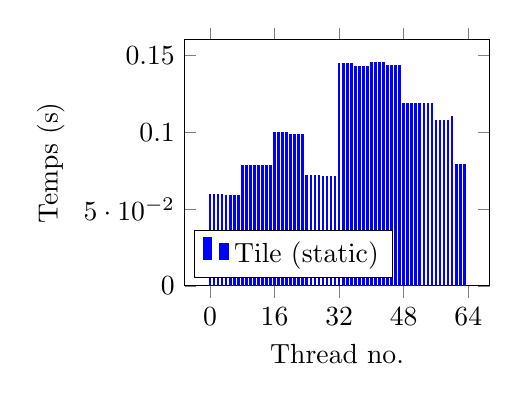
\begin{tikzpicture}
\begin{axis}[
  ybar,
  bar width=0.02cm,
  xlabel={Thread no.},
  ylabel={Temps (s)},
  ymin=0,
  legend pos=south west,
  width=0.45\textwidth,
  xtick distance=16
]

% Données pour le premier graphique (à gauche)
\addplot[color=blue, fill=blue] coordinates {
  (0,0.059273) (1,0.059272) (2,0.059272) (3,0.059272) (4,0.059028) (5,0.059030) (6,0.059028) (7,0.059026) (8,0.078182) (9,0.078182) (10,0.078183) (11,0.078183) (12,0.078179) (13,0.078179) (14,0.078179) (15,0.078179) (16,0.099472) (17,0.099473) (18,0.099470) (19,0.099469) (20,0.098562) (21,0.098562) (22,0.098562) (23,0.098562) (24,0.071909) (25,0.071909) (26,0.071912) (27,0.071911) (28,0.070826) (29,0.070828) (30,0.070826) (31,0.070826) (32,0.144565) (33,0.144566) (34,0.144566) (35,0.144565) (36,0.142607) (37,0.142604) (38,0.142607) (39,0.142602) (40,0.145585) (41,0.145585) (42,0.145587) (43,0.145588) (44,0.143405) (45,0.143406) (46,0.143401) (47,0.143403) (48,0.118553) (49,0.118567) (50,0.118648) (51,0.118552) (52,0.118556) (53,0.118660) (54,0.118556) (55,0.118578) (56,0.107295) (57,0.107289) (58,0.107289) (59,0.107312) (60,0.110412) (61,0.078990) (62,0.079167) (63,0.079191)
};
\addlegendentry{Tile (static)}

\end{axis}
\end{tikzpicture}
\hfill
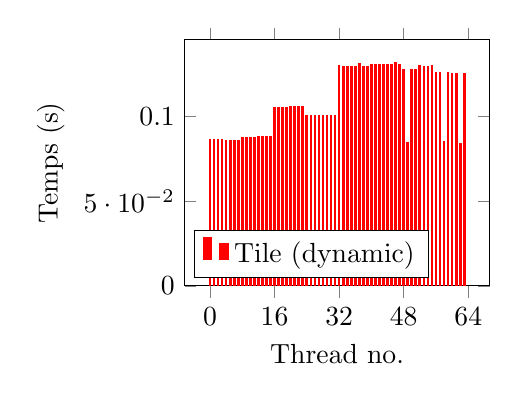
\begin{tikzpicture}
\begin{axis}[
  ybar,
  bar width=0.02cm,
  xlabel={Thread no.},
  ylabel={Temps (s)},
  ymin=0,
  legend pos=south west,
  width=0.45\textwidth,
  xtick distance=16
]

% Données pour le deuxième graphique (au milieu)
\addplot[color=red, fill=red] coordinates {
  (0,0.086742) (1,0.086742) (2,0.086744) (3,0.086743) (4,0.085574) (5,0.085574) (6,0.085574) (7,0.085574) (8,0.087906) (9,0.087906) (10,0.087906) (11,0.087906) (12,0.087957) (13,0.087957) (14,0.088018) (15,0.087957) (16,0.105483) (17,0.105482) (18,0.105483) (19,0.105522) (20,0.105897) (21,0.105830) (22,0.105830) (23,0.105830) (24,0.100408) (25,0.100408) (26,0.100408) (27,0.100408) (28,0.100795) (29,0.100796) (30,0.100795) (31,0.100795) (32,0.130219) (33,0.129782) (34,0.129782) (35,0.129782) (36,0.129814) (37,0.131139) (38,0.129814) (39,0.129899) (40,0.130673) (41,0.130673) (42,0.130674) (43,0.130674) (44,0.130935) (45,0.130935) (46,0.132224) (47,0.130935) (48,0.128009) (49,0.084798) (50,0.128014) (51,0.127863) (52,0.129916) (53,0.129900) (54,0.129900) (55,0.129906) (56,0.126044) (57,0.126046) (58,0.085242) (59,0.126048) (60,0.125719) (61,0.125640) (62,0.084154) (63,0.125632)
};
\addlegendentry{Tile (dynamic)}

\end{axis}
\end{tikzpicture}
\hfill
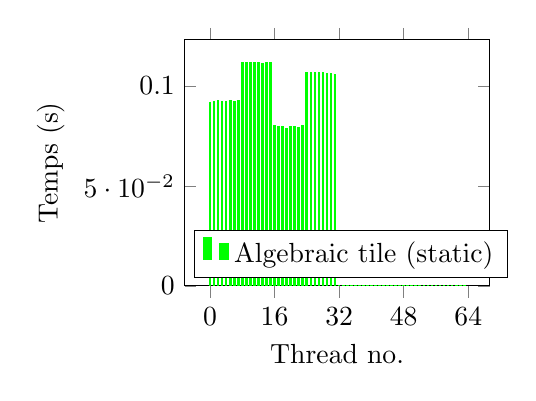
\begin{tikzpicture}
\begin{axis}[
  ybar,
  bar width=0.02cm,
  xlabel={Thread no.},
  ylabel={Temps (s)},
  ymin=0,
  legend pos=south west,
  width=0.45\textwidth,
  xtick distance=16
]

% Données pour le troisième graphique (à droite)
\addplot[color=green, fill=green] coordinates {
  (0,0.091535) (1,0.092345) (2,0.092657) (3,0.092319) (4,0.092400) (5,0.092443) (6,0.092217) (7,0.092637) (8,0.111836) (9,0.111764) (10,0.111806) (11,0.111858) (12,0.111884) (13,0.111195) (14,0.111716) (15,0.111828) (16,0.080034) (17,0.079513) (18,0.079488) (19,0.078850) (20,0.079775) (21,0.079856) (22,0.079379) (23,0.079923) (24,0.106595) (25,0.106652) (26,0.106427) (27,0.106832) (28,0.106440) (29,0.106097) (30,0.106066) (31,0.105864) (32,0.000060) (33,0.000059) (34,0.000058) (35,0.000058) (36,0.000060) (37,0.000061) (38,0.000061) (39,0.000061) (40,0.000063) (41,0.000062) (42,0.000062) (43,0.000061) (44,0.000061) (45,0.000062) (46,0.000061) (47,0.000062) (48,0.000060) (49,0.000060) (50,0.000060) (51,0.000060) (52,0.000061) (53,0.000061) (54,0.000061) (55,0.000061) (56,0.000062) (57,0.000062) (58,0.000062) (59,0.000062) (60,0.000062) (61,0.000062) (62,0.000062) (63,0.000062)
};
\addlegendentry{Algebraic tile (static)}

\end{axis}
\end{tikzpicture}

\caption{Temps d'exécution des threads pour le fichier mvt.c}
\label{fig:graphes}
\end{figure}

\begin{table}[htbp]
  \centering
  \caption{Statistiques pour le fichier mvt.c}
  \begin{tabular}{|c|c|c|c|}
    \hline
    Statistique & Algebraic Tile & Tile (static) & Tile (dynamic) \\ 
    \hline
    Skewness (g1)  & 0.0922342 & 0.181173 & -0.105451 \\ 
    Kurtosis (g2)  & -1.88313 & -1.36867 & -1.68497 \\ 
    Coefficient de variation $ \frac{\sigma}{\overline{x}} $ & 1.01515 & 0.299429 & 0.168488\\ 
    Percent Imbalance metric en \% & 129.345 & 43.5255 & 20.1403\\ 
    Coefficient de Gini  & 0.534954 & 0.16973 & 0.093082\\ 
    Temps d'exécution (s) &  0.112278    &  0.145702   &  0.132336   \\ 

    \hline
  \end{tabular}
\end{table}
g1=$ \frac{\sum_{i=1}^{n} (x_i - \overline{x})^3}{n\sigma^3} $\
g2=$ \frac{\sum_{i=1}^{n} (x_i - \overline{x})^4}{n\sigma^4} $\
Coefficient de Gini = $ \frac{\sum_{i=1}^{n}\sum_{j=1}^{n} |x_i - x_j|}{2n^2\overline{x}} $\
\newpage

\begin{figure}
\centering

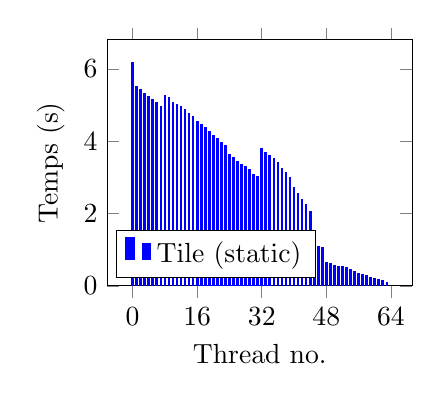
\begin{tikzpicture}
\begin{axis}[
  ybar,
  bar width=0.02cm,
  xlabel={Thread no.},
  ylabel={Temps (s)},
  ymin=0,
  legend pos=south west,
  width=0.45\textwidth,
  xtick distance=16
]

% Données pour le premier graphique (à gauche)
\addplot[color=blue, fill=blue] coordinates {
  (0,6.186381) (1,5.523618) (2,5.429559) (3,5.322836) (4,5.230887) (5,5.145374) (6,5.054861) (7,4.964847) (8,5.252253) (9,5.195186) (10,5.076321) (11,5.016496) (12,4.954090) (13,4.865256) (14,4.775598) (15,4.685738) (16,4.542174) (17,4.453248) (18,4.364084) (19,4.273877) (20,4.155637) (21,4.065181) (22,3.970165) (23,3.876787) (24,3.627207) (25,3.535051) (26,3.436402) (27,3.347539) (28,3.293050) (29,3.226376) (30,3.085248) (31,3.010873) (32,3.783154) (33,3.674158) (34,3.588986) (35,3.513408) (36,3.394945) (37,3.245654) (38,3.135966) (39,3.006817) (40,2.710400) (41,2.544449) (42,2.392712) (43,2.247311) (44,2.062699) (45,1.144879) (46,1.098367) (47,1.048379) (48,0.637953) (49,0.606421) (50,0.570815) (51,0.535764) (52,0.528368) (53,0.491483) (54,0.449944) (55,0.405056) (56,0.340516) (57,0.308230) (58,0.273170) (59,0.234820) (60,0.211501) (61,0.169822) (62,0.141123) (63,0.088914)
};
\addlegendentry{Tile (static)}

\end{axis}
\end{tikzpicture}
\hfill
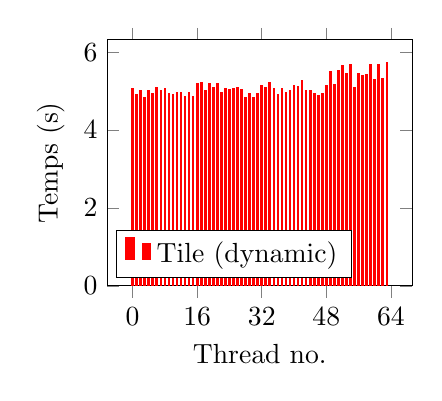
\begin{tikzpicture}
\begin{axis}[
  ybar,
  bar width=0.02cm,
  xlabel={Thread no.},
  ylabel={Temps (s)},
  ymin=0,
  legend pos=south west,
  width=0.45\textwidth,
  xtick distance=16
]

% Données pour le deuxième graphique (au milieu)
\addplot[color=red, fill=red] coordinates {
  (0,5.060731) (1,4.904975) (2,5.022152) (3,4.842046) (4,5.013940) (5,4.945685) (6,5.097318) (7,5.013807) (8,5.067446) (9,4.927886) (10,4.899633) (11,4.950998) (12,4.954185) (13,4.850294) (14,4.954710) (15,4.850529) (16,5.198048) (17,5.227108) (18,5.014245) (19,5.195400) (20,5.084436) (21,5.185327) (22,4.970609) (23,5.073412) (24,5.030226) (25,5.074391) (26,5.081033) (27,5.038400) (28,4.834552) (29,4.948605) (30,4.846230) (31,4.948744) (32,5.149949) (33,5.092741) (34,5.223701) (35,5.062466) (36,4.903681) (37,5.058218) (38,4.975679) (39,5.020903) (40,5.148468) (41,5.119003) (42,5.258816) (43,5.006288) (44,5.003373) (45,4.944955) (46,4.897579) (47,4.944937) (48,5.141304) (49,5.497010) (50,5.173397) (51,5.523123) (52,5.661881) (53,5.451412) (54,5.691668) (55,5.098905) (56,5.455075) (57,5.396348) (58,5.424860) (59,5.673018) (60,5.293196) (61,5.677864) (62,5.325166) (63,5.744917)
};
\addlegendentry{Tile (dynamic)}

\end{axis}
\end{tikzpicture}
\hfill
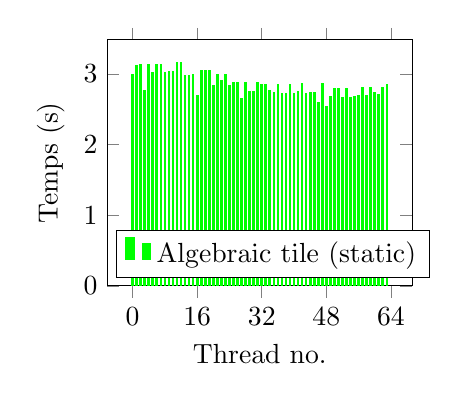
\begin{tikzpicture}
\begin{axis}[
  ybar,
  bar width=0.02cm,
  xlabel={Thread no.},
  ylabel={Temps (s)},
  ymin=0,
  legend pos=south west,
  width=0.45\textwidth,
  xtick distance=16
]

% Données pour le troisième graphique (à droite)
\addplot[color=green, fill=green] coordinates {
  (0,2.998546) (1,3.126950) (2,3.128272) (3,2.771574) (4,3.130790) (5,3.021602) (6,3.131411) (7,3.131273) (8,3.028297) (9,3.032184) (10,3.028745) (11,3.160513) (12,3.169210) (13,2.973068) (14,2.973142) (15,2.994333) (16,2.691778) (17,3.050416) (18,3.050757) (19,3.053299) (20,2.835243) (21,2.996952) (22,2.903801) (23,2.997117) (24,2.841502) (25,2.884907) (26,2.884984) (27,2.646748) (28,2.884738) (29,2.750741) (30,2.750904) (31,2.884578) (32,2.854836) (33,2.854476) (34,2.771061) (35,2.743511) (36,2.849266) (37,2.716991) (38,2.717071) (39,2.849395) (40,2.728819) (41,2.756364) (42,2.865830) (43,2.728924) (44,2.741631) (45,2.737743) (46,2.598702) (47,2.865264) (48,2.542404) (49,2.683218) (50,2.799617) (51,2.799875) (52,2.667592) (53,2.792567) (54,2.667494) (55,2.680847) (56,2.691107) (57,2.804123) (58,2.691569) (59,2.805168) (60,2.741999) (61,2.704789) (62,2.807559) (63,2.847428)
};
\addlegendentry{Algebraic tile (static)}

\end{axis}
\end{tikzpicture}

\caption{Temps d'exécution des threads pour le fichier correlation.c}
\label{fig:graphes}
\end{figure}

\begin{table}[htbp]
  \centering
  \caption{Statistiques pour le fichier correlation.c}
  \begin{tabular}{|c|c|c|c|}
    \hline
    Statistique & Algebraic Tile & Tile (static) & Tile (dynamic) \\ 
    \hline
    Skewness (g1)  & 0.347473 & -0.295629 & 1.13238 \\ 
    Kurtosis (g2)  & -0.839794 & -1.27959 & 0.459704 \\ 
    Coefficient de variation $ \frac{\sigma}{\overline{x}} $ & 0.0542904 & 0.613835 & 0.04532\\ 
    Percent Imbalance metric en \% & 10.8263 & 106.721 & 12.0457\\ 
    Coefficient de Gini  & 0.0307794 & 0.347492 & 0.0241421\\ 
    Temps d'exécution (s) &  3.255758    &  6.269201   &  5.765983   \\ 

    \hline
  \end{tabular}
\end{table}
g1=$ \frac{\sum_{i=1}^{n} (x_i - \overline{x})^3}{n\sigma^3} $\
g2=$ \frac{\sum_{i=1}^{n} (x_i - \overline{x})^4}{n\sigma^4} $\
Coefficient de Gini = $ \frac{\sum_{i=1}^{n}\sum_{j=1}^{n} |x_i - x_j|}{2n^2\overline{x}} $\
\newpage

\begin{figure}
\centering

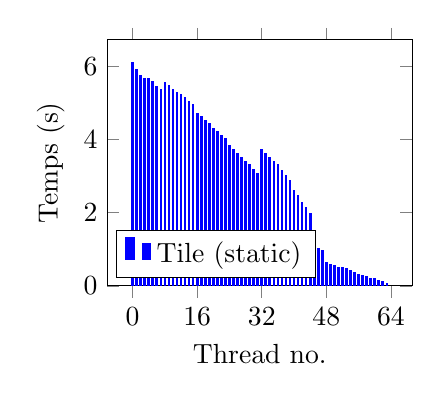
\begin{tikzpicture}
\begin{axis}[
  ybar,
  bar width=0.02cm,
  xlabel={Thread no.},
  ylabel={Temps (s)},
  ymin=0,
  legend pos=south west,
  width=0.45\textwidth,
  xtick distance=16
]

% Données pour le premier graphique (à gauche)
\addplot[color=blue, fill=blue] coordinates {
  (0,6.120425) (1,5.909225) (2,5.744122) (3,5.660519) (4,5.660238) (5,5.575614) (6,5.456981) (7,5.373776) (8,5.569097) (9,5.485814) (10,5.368115) (11,5.282857) (12,5.231237) (13,5.148990) (14,5.029219) (15,4.946187) (16,4.725037) (17,4.640770) (18,4.521360) (19,4.436361) (20,4.313048) (21,4.233856) (22,4.106863) (23,4.021156) (24,3.833565) (25,3.723842) (26,3.617269) (27,3.507695) (28,3.411603) (29,3.315312) (30,3.183705) (31,3.084495) (32,3.731561) (33,3.606659) (34,3.508336) (35,3.400777) (36,3.309854) (37,3.154215) (38,3.027061) (39,2.889799) (40,2.612851) (41,2.464060) (42,2.289931) (43,2.150838) (44,1.976356) (45,1.059525) (46,1.005664) (47,0.953413) (48,0.626395) (49,0.591225) (50,0.552162) (51,0.512093) (52,0.500774) (53,0.461352) (54,0.415985) (55,0.369231) (56,0.318541) (57,0.281972) (58,0.243293) (59,0.201760) (60,0.186216) (61,0.141194) (62,0.110289) (63,0.070285)
};
\addlegendentry{Tile (static)}

\end{axis}
\end{tikzpicture}
\hfill
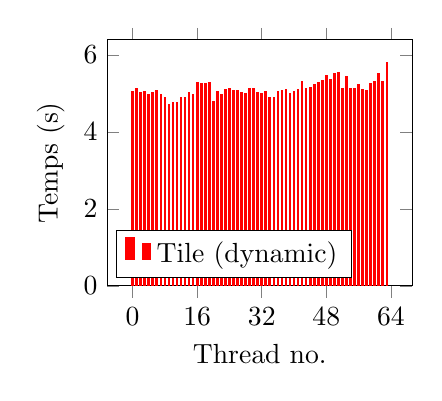
\begin{tikzpicture}
\begin{axis}[
  ybar,
  bar width=0.02cm,
  xlabel={Thread no.},
  ylabel={Temps (s)},
  ymin=0,
  legend pos=south west,
  width=0.45\textwidth,
  xtick distance=16
]

% Données pour le deuxième graphique (au milieu)
\addplot[color=red, fill=red] coordinates {
  (0,5.054511) (1,5.135593) (2,5.020645) (3,5.055130) (4,4.959677) (5,5.018882) (6,5.078414) (7,4.959471) (8,4.901221) (9,4.718431) (10,4.770809) (11,4.770712) (12,4.902427) (13,4.902467) (14,5.014600) (15,4.962807) (16,5.282258) (17,5.249551) (18,5.249471) (19,5.282263) (20,4.773744) (21,5.052094) (22,4.971236) (23,5.098997) (24,5.119768) (25,5.081610) (26,5.081538) (27,5.015251) (28,4.986923) (29,5.135069) (30,5.135025) (31,5.022816) (32,5.003767) (33,5.046216) (34,4.897819) (35,4.897978) (36,5.038009) (37,5.071921) (38,5.102807) (39,4.989872) (40,5.050032) (41,5.090712) (42,5.309468) (43,5.124516) (44,5.152623) (45,5.215760) (46,5.279311) (47,5.341201) (48,5.470701) (49,5.357557) (50,5.502734) (51,5.537073) (52,5.123738) (53,5.436287) (54,5.123609) (55,5.123696) (56,5.234918) (57,5.107392) (58,5.065000) (59,5.261074) (60,5.298710) (61,5.508907) (62,5.298794) (63,5.811024)
};
\addlegendentry{Tile (dynamic)}

\end{axis}
\end{tikzpicture}
\hfill
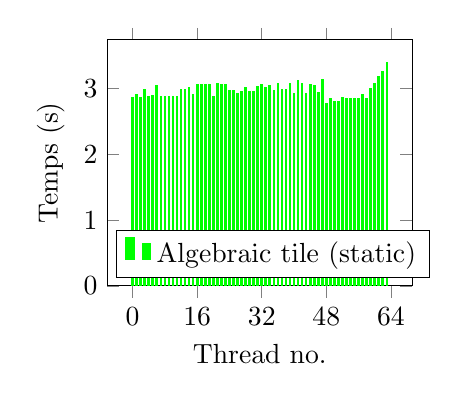
\begin{tikzpicture}
\begin{axis}[
  ybar,
  bar width=0.02cm,
  xlabel={Thread no.},
  ylabel={Temps (s)},
  ymin=0,
  legend pos=south west,
  width=0.45\textwidth,
  xtick distance=16
]

% Données pour le troisième graphique (à droite)
\addplot[color=green, fill=green] coordinates {
  (0,2.865332) (1,2.911932) (2,2.871403) (3,2.994229) (4,2.885102) (5,2.901220) (6,3.051900) (7,2.886485) (8,2.876559) (9,2.879067) (10,2.876247) (11,2.873221) (12,2.981174) (13,2.980947) (14,3.015675) (15,2.912512) (16,3.059921) (17,3.061409) (18,3.060575) (19,3.060311) (20,2.882402) (21,3.072531) (22,3.060799) (23,3.061139) (24,2.975905) (25,2.976108) (26,2.930402) (27,2.952559) (28,3.025012) (29,2.960517) (30,2.960881) (31,3.025983) (32,3.056422) (33,3.015227) (34,3.055184) (35,2.971776) (36,3.080374) (37,2.990468) (38,2.990587) (39,3.080519) (40,2.922424) (41,3.131580) (42,3.078297) (43,2.922744) (44,3.062533) (45,3.044659) (46,2.936000) (47,3.131859) (48,2.768377) (49,2.844223) (50,2.802914) (51,2.802887) (52,2.864126) (53,2.857458) (54,2.857703) (55,2.857593) (56,2.850431) (57,2.908964) (58,2.851025) (59,3.004612) (60,3.082071) (61,3.178479) (62,3.256767) (63,3.404628)
};
\addlegendentry{Algebraic tile (static)}

\end{axis}
\end{tikzpicture}

\caption{Temps d'exécution des threads pour le fichier covariance.c}
\label{fig:graphes}
\end{figure}

\begin{table}[htbp]
  \centering
  \caption{Statistiques pour le fichier covariance.c}
  \begin{tabular}{|c|c|c|c|}
    \hline
    Statistique & Algebraic Tile & Tile (static) & Tile (dynamic) \\ 
    \hline
    Skewness (g1)  & 0.907532 & -0.223291 & 0.76719 \\ 
    Kurtosis (g2)  & 1.82569 & -1.33165 & 1.23447 \\ 
    Coefficient de variation $ \frac{\sigma}{\overline{x}} $ & 0.0378124 & 0.636624 & 0.0389099\\ 
    Percent Imbalance metric en \% & 14.3498 & 98.8746 & 13.5116\\ 
    Coefficient de Gini  & 0.0205509 & 0.362263 & 0.021061\\ 
    Temps d'exécution (s) &  3.419980 &  6.170514   &  5.825840   \\ 

    \hline
  \end{tabular}
\end{table}
g1=$ \frac{\sum_{i=1}^{n} (x_i - \overline{x})^3}{n\sigma^3} $\
g2=$ \frac{\sum_{i=1}^{n} (x_i - \overline{x})^4}{n\sigma^4} $\
Coefficient de Gini = $ \frac{\sum_{i=1}^{n}\sum_{j=1}^{n} |x_i - x_j|}{2n^2\overline{x}} $\
\newpage

  \end{document}
